\chapter[Study 3: Application of SPARC to Tutoring]{Study 3: \\Application of SPARC to Tutoring}\label{chap:tutoring}
\glsresetall
\graphicspath{{images/tutoring/}}

\begin{framed}
	\textbf{Key points:}
	
	\begin{itemize}
		\item Design of an experiment to test \acrshort{sparc} in an educative application with children.
		\item Design and use of a new learning algorithm adapted from nearest neighbours to teach quickly and efficiently in an online fashion.
		\item Between participants study involving 75 children comparing 3 conditions: a passive robot, a supervised robot and an autonomous robot.
		\item Psychology PhD student teaching the supervised robot using \acrshort{sparc}.
%		\item No significant differences of child learning between conditions.
		\item Similar children behaviours with the autonomous and supervised robot, and different to the passive robot.
		\item Demonstration of the applicability of \acrshort{sparc} to teach a robot online an action policy to interact with humans in a complex, indeterministic, high dimensional, multimodal and social space.
	\end{itemize}
\end{framed}

Parts of the work presented in this chapter have been published verbatim in \cite{senft2017toward} and \cite{senft2018robots}, an additional publication is under review. The final publications are available from AAAI, EPFL via:
\begin{itemize}
	\item \url{https://aaai.org/ocs/index.php/FSS/FSS17/paper/view/16011}.
	\item \url{https://r4l.epfl.ch/files/content/sites/r4l/files/HRI2018/proceedings_2018/paper4.pdf}.
\end{itemize} 

Technical contribution in this chapter: the author extended code the freeplay sandbox, see \url{https://github.com/freeplay-sandbox/} and forks.

\newpage

\section{Motivation}

Chapters~\ref{chap:woz} and~\ref{chap:control} tested the \gls{sparc} in interactions between robots or in a virtual world but not for \gls{hri} as it was intended to be used. As such, this Chapter addresses the thesis of this research and evaluates if \gls{sparc} can efficiently be used to teach a robot an interactive behaviour for real human-robot interactions. \gls{hri} in the wild typically occur in constrained but underspecified environments where social behaviours play an important role. Teaching a robot in such an environment is a challenge as the state and action spaces are of high dimension, the environment is not deterministic, the interaction takes place in continuous time and is multimodal; and finally, the social side is fundamental as it impacts the flow and the success of the interaction.

This study takes place in the context of robot tutors for children in education. Tutoring is a framework widely used in \gls{hri} and providing opportunities for a rich and complex interaction between a child and a robot~\citep{leyzberg2012physical,kennedy2015robot}. This scenario and the code are based on \cite{lemaignan2017free} but have been adapted to provide a new teaching task (teaching game and protocol), a knowledge test, a specific robot controller, a learning algorithm and an interface with the teacher supporting \gls{sparc}.

%This study aims to explore if \gls{sparc} can be used to teach a robot an efficient action policy. As such, three conditions have been compared: a passive robot (not providing any support), a supervised robot (learning from a human teacher and supporting the child) and an autonomous robot (applying the learned behaviour). These three conditions, with the passive robot as a control condition, allow us to study both the teaching process and the efficiency of the taught behaviour when being executed without supervision.

\section{Scope of the Study} \label{sec:tutoring_scope}

The main goal of this study was to explore the thesis proposed in this work: ``A robot can learn to interact meaningfully with humans in an efficient and safe way by receiving supervision from a human teacher in control of the robot's behaviour''. This thesis can be divided into two parts: ``a robot can learn safely by receiving supervision from a human teacher'' and ``after learning, such a robot would have a meaningful interaction with humans''. To address these two statements, a study comparing three conditions was designed. 

The focus of the study is on the behaviour of the robot, not its impact compared to another agent or none. As such, to prevent confounds about novelty effect and potential excitements due to the robot, the control condition maintained the robot through all the interaction. In the control condition, the `passive' condition, the robot guide the child in the task as in the other conditions, but is not interacting with the child during the learning game. This condition provides a benchmark against which the other conditions can be compared to evaluate the `meaningfulness' and efficiency of the robot's behaviour. In the second condition, the `supervised' condition, the robot is being supervised and taught by a human teacher using \gls{sparc}. This condition is the one in which the robot learns, and can be used to evaluate the impacts of the principles underlying \gls{sparc} when teaching a robot to interact with humans. Lastly, in the `autonomous' condition, the robot applies the learnt policy to interact without supervision with the children. This condition aims at exploring how different the autonomous policy is from the supervised one, and evaluating if the teaching from the human was successful. And as the robot needed to have completed its learning before interacting alone, this condition was run only after the supervised condition was completed.

These conditions allowed us to explore the statements presented above through three hypotheses:
\begin{itemize}
	\item [H1] The autonomous robot is able to interact socially and efficiently during the game sessions and maintain the child's engagement during the learning task.
	\item [H2] An active robot (supervised or autonomous) supports child learning: learning gain in passive condition $<$ learning gain in autonomous condition $<$ learning gain in supervised condition.
	\item [H3] Using \gls{sparc}, the workload on the supervisor decreases over time: the number of corrected actions and the number of actions selected  by the teacher decrease with the progress in the sessions, while the number of correct proposed actions increases.
\end{itemize}

\section{Methodology}

\subsection{Participants}

Children from five classrooms from two different schools in Plymouth were recruited to take part in the study. As both schools have an identical OFSTED evaluation (both school ``require improvement''), so all the children were combined into a single pool of participants. Full permission to take part in the study and be recorded on video was acquired for all the participants. In total, 119 children participated in the study, however not all of them have been included in the final analysis. Some participants took part in two pilot versions, with previous versions of the game or the protocol. For other participants, a breach in the protocol have prevented them to be included (such as freezing of the tablet due to an imperfect kernel version or refusing to continue the interaction). Additionally, children with special needs were encouraged to participate but were not included in the results. In the end, 25 participants per condition were included (N=75 in total; age: \textit{M}=9.4, \textit{SD}=0.72; 37F/38M). The remaining children in the classrooms interacted by pairs (and were not included in the evaluation) to accelerate the ending of the study, and free the room used in the school while giving to each child the opportunity to interact with the robot. 

\subsection{Setup of the study}

Similarly to the study presented in Chapter~\ref{chap:woz}, this study is based on the Sandtray paradigm~\citep{baxter2012touchscreen}: a child interacts with a robot through a large touchscreen located between them and by interacting with the touchscreen and the robot, the child is expected to gain knowledge or improve some skills. Additionally, a teacher can use a tablet to control and teach the robot in the `supervised' conditions (cf. Figure~\ref{fig:tutoring_setup}). This type of potentially triadic interaction is typical of the interactions we considered when framing this research (cf. Figure~\ref{fig:intro_setup}). We desire an efficient behaviour for the robot in the application interaction (i.e. child tutoring) and a human teacher has knowledge about how the robot should behave and can transfer it to the robot in situ by using \gls{sparc}.

\begin{figure}[ht]
	\centering
	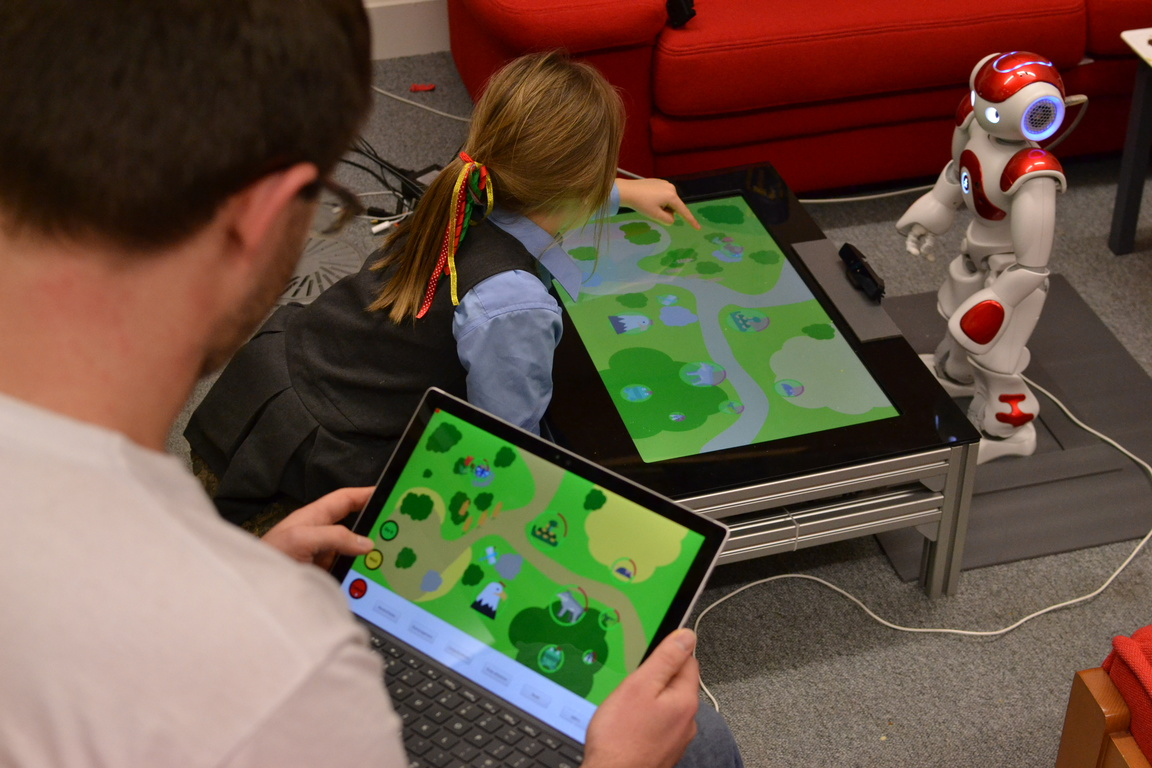
\includegraphics[width=1\textwidth]{setup.jpg}
	\caption{Setup used in the study: a child interacts with the robot tutor, with a large touchscreen sitting between them displaying the learning activity; a human teacher provides supervision to the robot through a tablet and monitors the robot learning.}
	\label{fig:tutoring_setup}
\end{figure}

By interacting with the robot and the sandtray, the child is expected to gain knowledge on a specific topic. For this study, the task is learning about food chains by exploring a specific food web (interconnections between multiple food chains) in an educative game. The child plays a game on the sandtray where they can move animals to discover the interactions between them. Learning is evaluated by a test before, between and after the sessions; and the robot guides the child through the study and can, depending of the condition, support them during the game.

\subsection{Food Chain Game}

The main learning activity to teach the child the food web is a game composed of ten animals and three types of plants (with a total of 11 instances of plant in the game: 4 wheat, 4 apples and 3 flowers). Animals have energy decreasing over time and they have to eat to stay healthy. Animals are not moving unless the child or the robot moves them and can eat or be eaten when entering in contact with another animal or a plant. The child has to feed the animals by moving them to their food to give them more energy and by feeding the animals, children should learn the animals' diet. Figure~\ref{fig:tutoring_game} presents an example of the game screen in the middle of a session. The children are instructed to keep the animals alive as long as possible

\begin{figure}[ht]
	\centering
		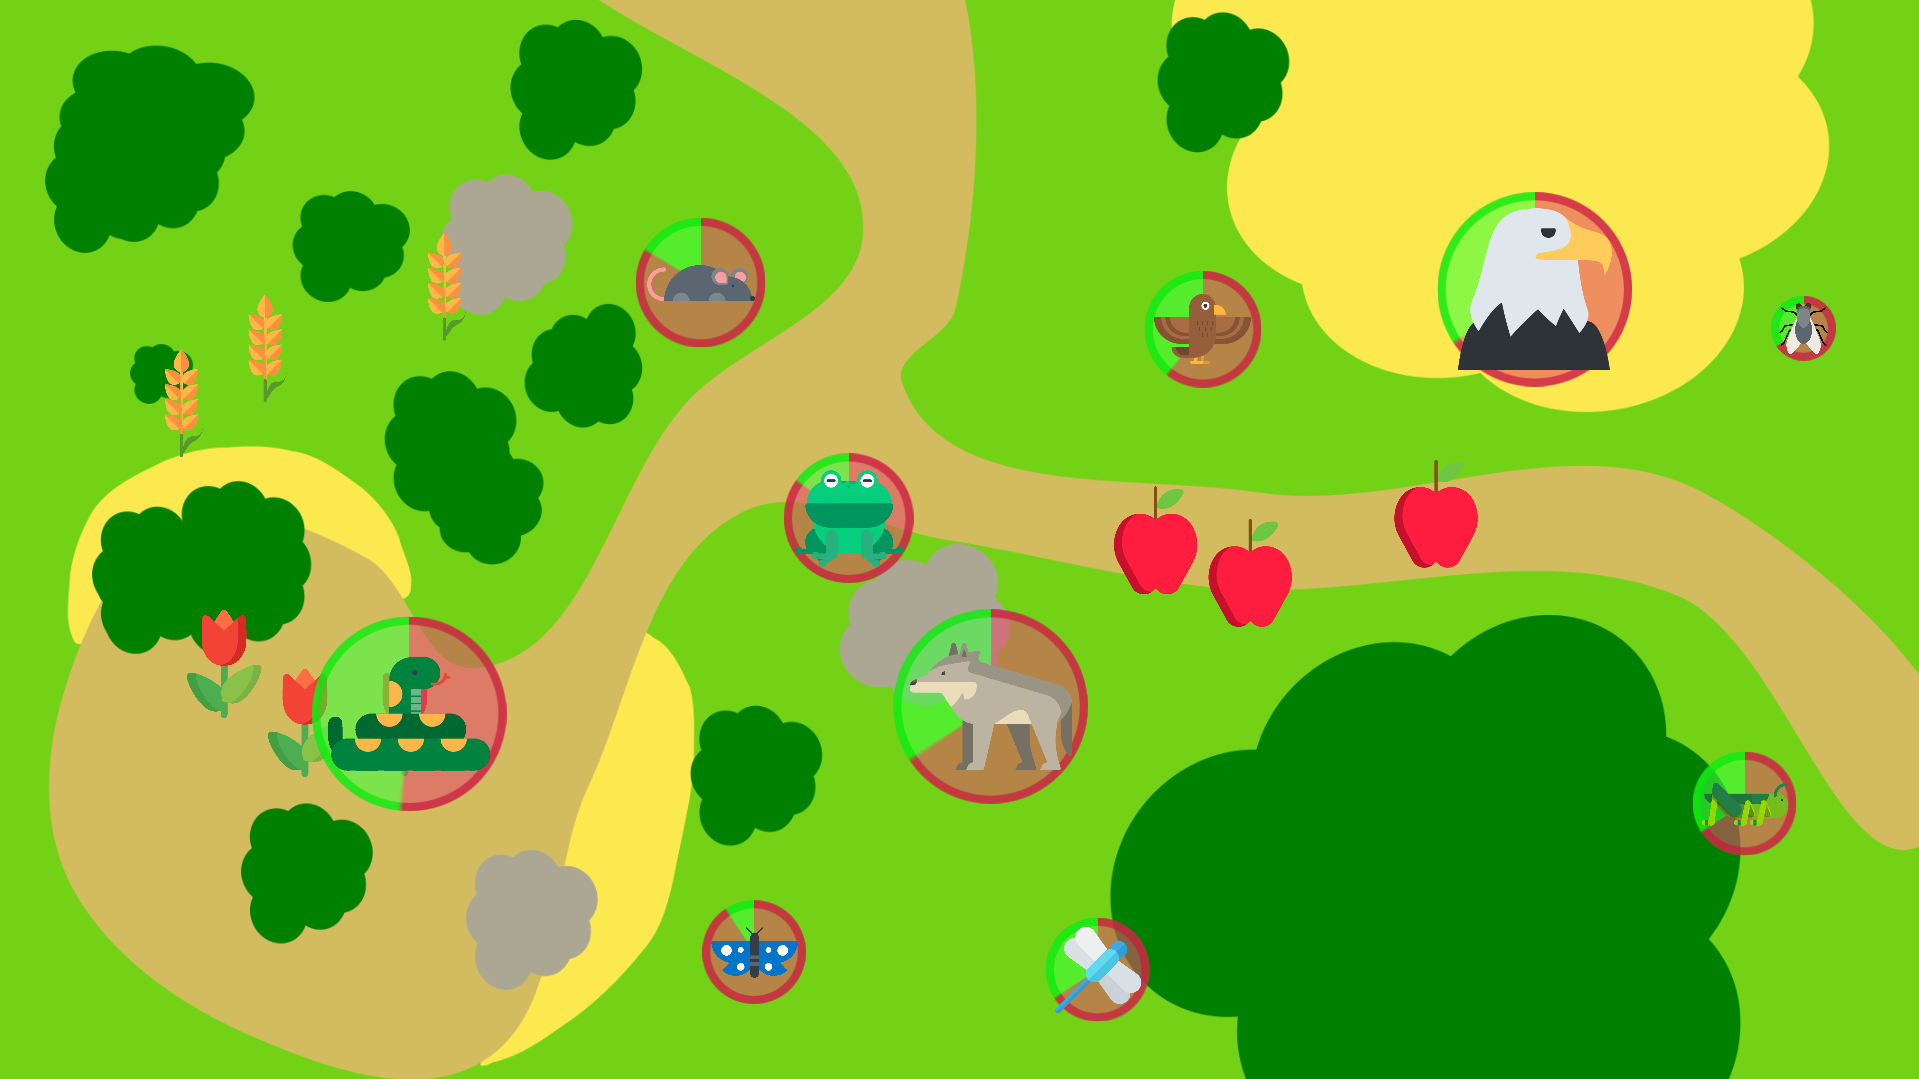
\includegraphics[width=1\textwidth]{game.png}
		\caption{Example of the game. Animals have energy in green and have to eat plants or other animals to survive. The child's task is to keep animals alive as long as possible.}
		\label{fig:tutoring_game}
\end{figure}

\subsection{Robot Behaviour}
 
During the game, the robot can execute actions to provide hints and support to the child. The robot has access to five types of actions:
\begin{itemize}
	\item Movements: moving any animal to, close to or away from any items (animal or plant) - the robot points to an animal and moves it on the game while describing its action (e.g. "The eagle needs help getting close to the mouse").
	\item Drawing attention: the robot points an item and says a reminder to the child (e.g. "Don't forget the frog").
	\item Reminding rules: the robot says one of 5 sentences describing the game's rules (e.g. "Move the animals to feed them" or "Feed animals with a low energy").
	\item Congratulation: the robot provides congratulations (e.g. "Well done").
	\item Encouragement: the robot provides encouragement (e.g. "You can do it").
\end{itemize}
Considering all the possible combinations of actions and items, the total number of actions adds up 655. Additionally, to prevent the robot's behaviour to be repetitive and annoying, each utterance joining an action has multiple versions, and a random one not used recently is selected. 

This set of actions has been selected to be generalisable to many type of scenario including a teaching activity on a screen. Furthermore, in this study, these actions represent different level of support, from general motivation and information on the game's goal to which animals the child should focus on or direct information about what an animal eats. This selection of actions aims to cover a large range of possible tutoring behaviours humans could use. 

\subsection{Wizard of Oz Application}

In this study, the communication between the teacher and the robot occurs through the \gls{woz} application, a \gls{gui} running on a tablet and allowing the teacher and the robot to communicate. This \gls{gui} represents the state of the game as the child sees it, but with additional button and functionalities to communicate both ways with the robot (see Figure~\ref{fig:tutoring_gui}). The teacher can use a combination of buttons and moving animals on the tablet to have the robot execute any possible action. For example, to move animals close to another item, the teacher can drag and release the animal's image to a position to request the robot to execute this movement. The robot controller will infer which action has been selected by the teacher by evaluating how the distances between animals change. Additionally, the teacher can select other animals or plants to clarify their action and give information to the learning algorithm about what features were relevant in the decision process. Similarly, the teacher can select an animal and press the `Draw attention' button to have the robot point at the select animal and remind the child to use it.
%The main aim of the study being testing \gls{sparc} in a real \gls{hri}, the teacher needs an interface to communicate with the robot. To allow this interaction between the teacher and the robot, a \gls{gui} running on a tablet has been developed representing the current state of the game exactly as the child sees it on the touchscreen (see in Figure~\ref{fig:tutoring_gui}). This \gls{gui} runs on a tablet as it allow the robot's teacher to supervise and teach the robot while monitoring the application interaction (i.e. the interaction between the child and the robot). Buttons for the actions (excluding movements) allow the teacher to select which action the want the robot to execute. The teacher can also have the robot move animals simply by dragging and releasing animals' images on the tablet. The teacher can also select animals or plants to specify which action they intend to do. 
For instance, by clicking on the frog and the `Draw attention' button, the robot will execute the \textit{drawing attention to the frog} action. 
%Similarly, the moving action require two items: the animal moved and the target of the motion. By selecting a target before moving an animal, the teacher can be sure that the robot interpret the action correctly. 
This \gls{gui} design gives access to the teacher to the full 655 actions without requiring as many buttons. %Additionally, the selection of items is used by the robot controller to identify the relevant features to transmit to the algorithm for the learning.

\begin{figure}[ht]
	\centering
	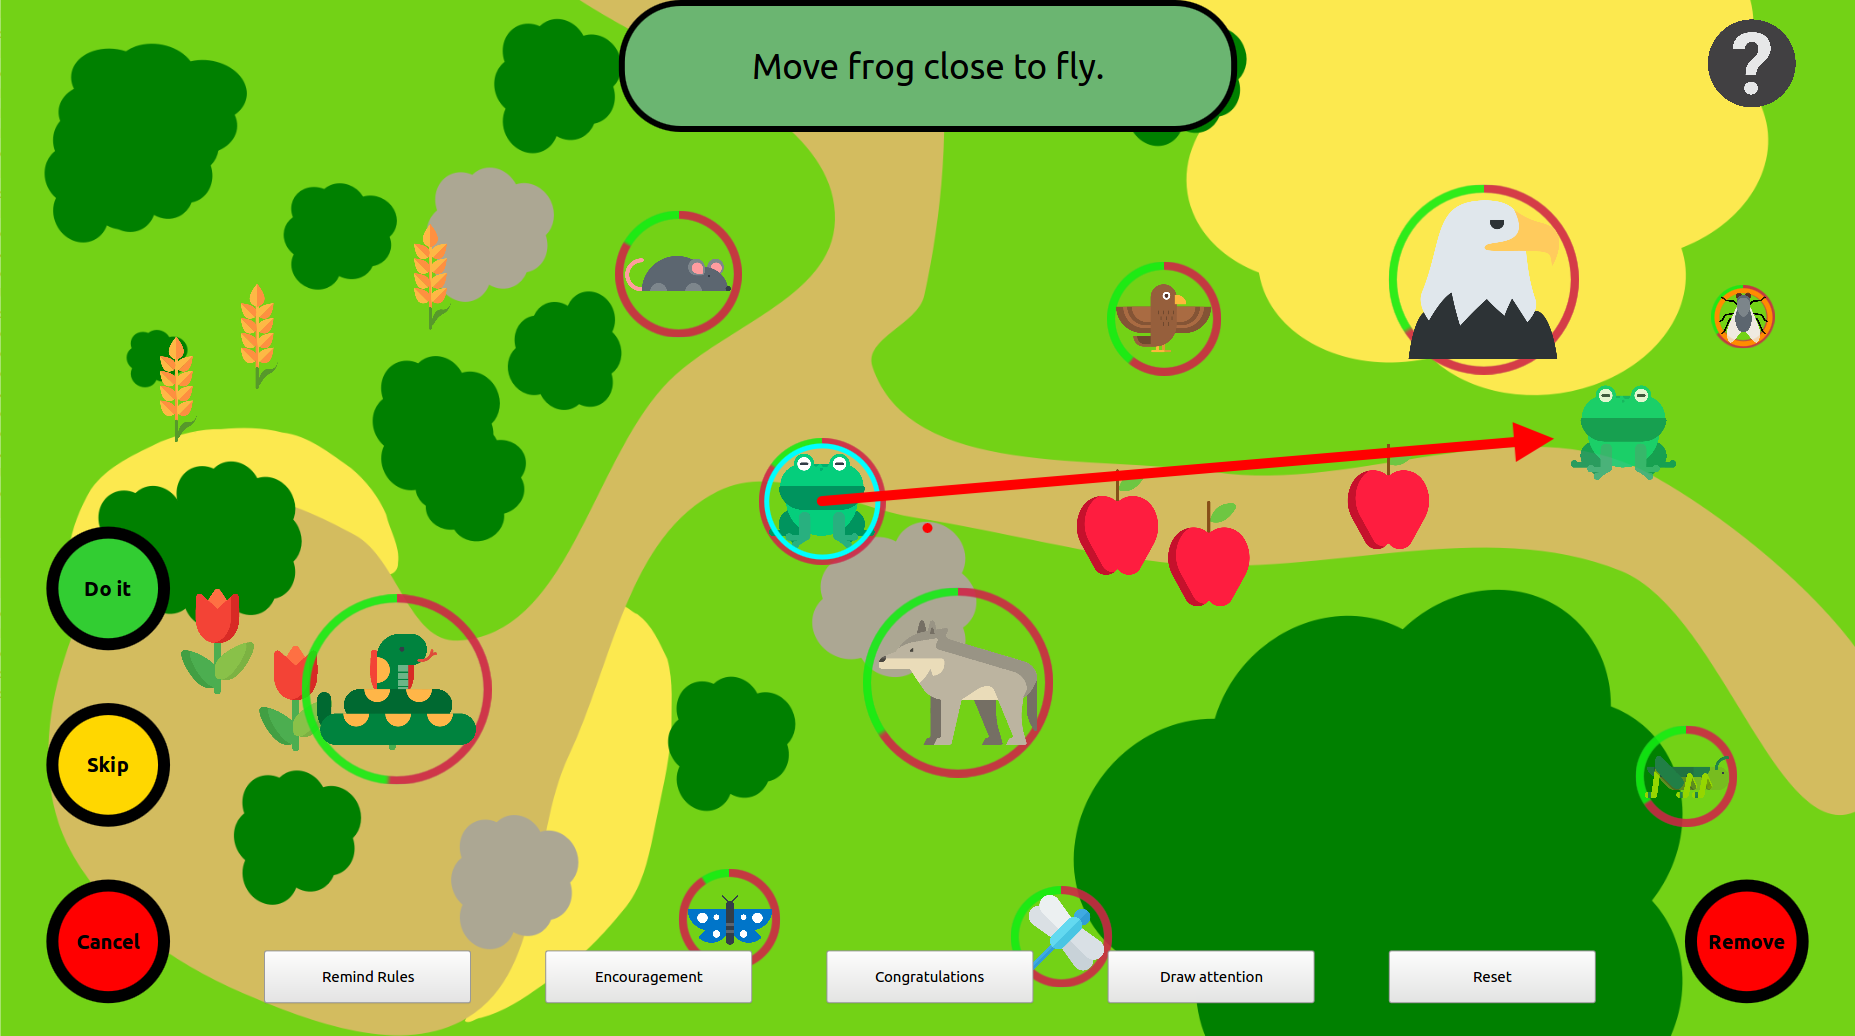
\includegraphics[width=1\textwidth]{gui.png}
	\caption{\gls{gui} used by the teacher to control the robot and respond to its suggestions. The game is in the same state as in Figure~\ref{fig:tutoring_game}, and the robot proposes to move the frog close to the fly (text bubble, arrow, moving the \textit{shadow} of the frog and highlight the frog and the fly).}
	\label{fig:tutoring_gui}
\end{figure}

Finally, the \gls{gui} is also used by the teacher to respond to the robot's propositions. Following the proposition of an action, a bubble describing the action will appear on top of the \gls{gui}, the corresponding items will be highlighted and if the action is a motion, an arrow will show the proposed motion. The teacher can react to the proposed action by pressing the `Do it', `Skip', `Cancel' or `Remove' buttons or let the action be executed. The action will be automatically executed after 2 seconds, during which the bubble will become greener to represent the passive acceptance of the action. The `Do it' button executes the action straight-away, the `Skip' button sends the `wait' action with a reward of 1, the `Cancel' sends the action with a -1 reward and does not execute it, and finally, the `Remove' button looks for the closest previous instantiation of the action in memory and removes it, preventing this instance to be used in later action selection. In each cases, by using buttons or automatic execution, the feature highlighted when the button is pressed (often the same as the one proposed by the algorithm) are sent with the action. Action executed by the robot (through `Do it', automatic execution or selection) are assigned a reward of 1.

\subsection{Control Architecture}

The code used to create the game and control the robot is an adaptation of the Freeplay Sandbox~\citep{lemaignan2017free}. Original sources are available online\footnote{\url{https://github.com/freeplay-sandbox}} as well as the code used for this study\footnote{\url{https://github.com/emmanuel-senft/freeplay-sandbox-qt/tree/food-chain}}\footnote{\url{https://github.com/emmanuel-senft/freeplay-sandbox-ros-sparc/tree/task}}\footnote{\url{https://github.com/emmanuel-senft/freeplay-sandbox-qt-supervisor}}.

The control architecture is adapted from \cite{lemaignan2017free} and a simplified schematic is presented in Figure~\ref{fig:tutoring_arch}. All nodes are communicating through ROS and the communication with the robot is done through NAOQI. The tool rosbag is used to collect data throughout the interaction and the analysis of the child's focus of attention is performed using gazr~\citep{lemaignan2016real}.

\begin{figure}[ht]
	\centering
	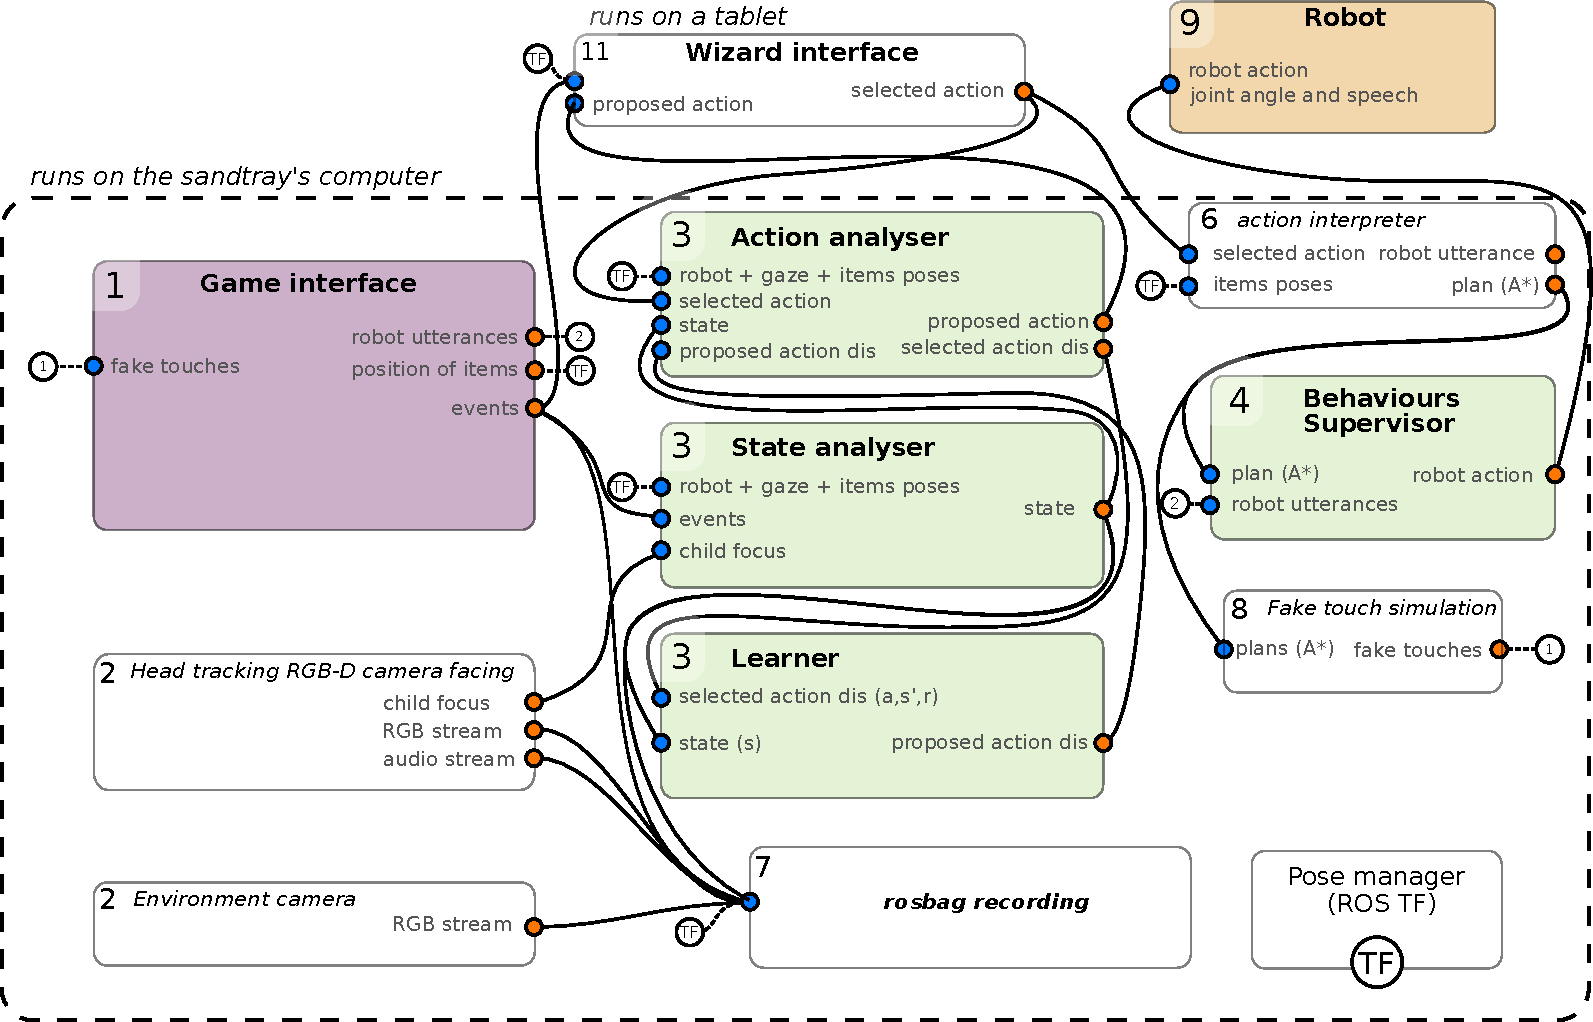
\includegraphics[width=1\textwidth]{architecture.pdf}
	\caption{Simplified schematics of the architecture used to control the robot. In addition, all the topics related to the actions are recorded using rosbag. (Figure adapted from \cite{lemaignan2017free}).}
	\label{fig:tutoring_arch}
\end{figure}

%Two worlds are cohabiting, the continuous world (as perceived by the child and the teacher) and the discrete world (as perceived by the algorithm). In the continuous world, actions are 

\ES{could add something about discrete vs continuous world, transformation of action and feature selection}

\subsection{Learning and Action Selection}

To learn and act autonomously, the robot has access to a representation of the state and a set of actions it can do and the algorithm aims at finding the ideal action for each possible state based on the teacher's commands.

\subsubsection{State}

Table~\ref{tab:tuto_state_space} presents the different dimensions composing the state the robot has access to.

\begin{table}[ht]
	\centering
	\ra{1.2}
	\caption{Definition of each category of the state space.}
	\label{tab:tuto_state_space}
	\begin{tabularx}{\textwidth}{@{}llX@{}}\toprule
		Name & Number & Description \\
		\midrule
		Distance between items & 155 & Normalised distance between the animals and each other animal and the plants\\
		Items' energy & 21 & Energy of the 21 items(10 animals and 11 plants)\\
		Time since robot touches & 10 & Time since the robot touched each animal\\ %decay
		Time since child touches & 10 & Time since the child touched each animal\\ %accumulation
		Progress in the game & 1 & 0.25 for 1st game to 1 for the last game\\ 
		Generic events & 3 & Time since last feeding, failed interaction and death of an animal\\ %decay
		Last robot's actions & 5 & Time since last type of robot action\\ %decay
		Generic last action & 2 & Time since any child touch and robot action\\ %decay\accumulation
		Focus & 3 & Time of focus toward the robot, the screen and outside\\ %accumulation
		\bottomrule
	\end{tabularx}
\end{table}

All the state values were bounded by [0,1]. Distances between items were normalised with the maximum possible distance (the diagonal of the screen), as there are 21 items (10 animals and 21 plants) this results in a total of 155 possible distances between items. To include a representation of the temporal aspect of the interaction, some dimensions represent the time since events and two methods have been used to transform the time since an event to a value bounded between 0 and 1:
\begin{itemize}
	\item Accumulation: for the times since child touches and focus (effect being true or false).
	\item Decay: for robot actions and touches and generic events (discrete events).
\end{itemize}

The accumulation corresponds to effect that can be true or not, and aims at representing how long this effect as been true or false. When the effect is true for accumulation, the state value is set to 0.5 and increases each step (by $1-e^{-\frac{1}{10}}$ of the missing value). And when the condition is false, the value is set to 0.5 and decreases (by being multiplied by $e^{-\frac{1}{10}})$ at each step. On the other hand the decay refers to discrete events, so only the time since the happened is relevant. When the event happens the corresponding state value is set to 1 and then exponentially decreases by being multiplied by $e^{-\frac{1}{10}}$. That way event will have a `half-life' of 7 steps, which corresponds to 3.5 seconds.

Parts of the states are hardcoded, such as the the generic events, generic last actions, focus and progress in the game. However, all the state dimensions related to the items (distance, energy and time since touches) are constructed on the fly. At start up, the state analyser node (cf. Figure~\ref{fig:tutoring_arch}), the node responsible for computing the state receives a list of the moving items and one of the immobile items and it creates the appropriate state with the corresponding dimensions. During the game, the state values are updated using events related to specific item (through their name). Additionally, each instance of a plant is considered as a unique element. For example, there are four instances of wheat, however each one is considered uniquely as a non-moving image and its type is not taken into account. It could have been possible to group the instances by categories, but it would require some add-hoc coding, limiting the generalisation of the approach. 

The state dimensions have been selected to be generic to many teaching tasks involving movable items: each item has a value assigned to it (here energy, but this could be changed in other scenario), and some items can be moved (here animals) while other are immobile. These dimensions represent both elements that define the state of the game itself, but also events around which a social policy could be constructed. For example, the events: last feeding and last failed interaction could be interpreted as a successful and a failed action from a child and trigger each different social response from the robot. While having a semantic interpretation for humans, the state does not represent them as a positive or a negative event, but only as two dimensions of the state that could be used to select actions. Using these generic this state definition, this implementation could be easily repurposed to another teaching task. New events would have to be defined,but to adapt the control to other items, their names would only have to be communicated, without any change in the code.
\ES{not clear, but the idea is that all the semantic interpretation of the dimensions and event is inferred from the demonstrations, without being hardcoded}

\subsubsection{Actions}

Table~\ref{tab:tuto_actions_space} present the list of actions used for this activity.

\begin{table}[ht]
	\centering
	\ra{1.2}
	\caption{Definition of each category of the action space.}
	\label{tab:tuto_actions_space}
	\begin{tabularx}{\textwidth}{@{}llX@{}}\toprule
		Name & Number & Description \\
		\midrule
		Move close & 210 &  Action moving any animal close to any item\\
		Move to & 210 & Action moving any animal to any item\\
		Move away & 210 & Action moving any animal away from any item\\
		Remind rules & 1 & \\
		Congratulation & 1 & \\
		Attention & 21 & Drawing attention to any item\\
		Encouragement & 1 & \\
		Wait & 1 & Doing nothing\\
		\bottomrule
	\end{tabularx}
\end{table}

The total action space available is 655 actions. Each move action is composed of 210 possibilities as we have a total of 10 animals which can be moved in relation to each animal (10) and each plant (11), which resuts in 210 actions for moving close, 210 for moving to and 210 for moving away. It should be noted that technically 30 actions exist but cannot be selected by the teacher (moving animals to/close to/away from themselves). But this does not impact the learning as an instance based algorithm is used. Similarly to the states, each instances of a same category (such the different images of the wheat) is considered as a unique non-moving item to create actions without any semantic interpretation.

In the same way as the state definition, this action space has been selected to be general to many activities including movable and immobile images. The robot has access to a wide range of actions, and the action space not includes little semantic specific to this game. For example, many of actions are available even if they are not relevant in this specific game (such as moving close together two unrelated animals). That way, some actions are game related and encompass the semantic knowledge of the game (such as which animal should be moved close to which one), other are more social, such as reminding the rules or encouraging feedback and some should simply be avoided as they could create confusion for the child. So, without have access to any semantic of the actions, the robot needs to learn which action are relevant to the task and when they should be executed.

The action interpreter node selects the precise utterance to join to an action, and this node would have to be modified when adapting to a new activity. However, similarly to the state, the actions related to items are generated at run time, and could be adapted to another activity with minimal or no change of the code. 

\ES{discuss the fact that limited semantic interpretation is used to define the action space - many not relevant actions, but even without this semantic information the robot can still learn an efficient action policy + if repurposed, no need to add additional semantic knowledge, the algo does it autonomously, and is non sensitive to the number of actions in the state}

%By using a generic definition of the action space, for example allowing to move close to each other two animals unrelated, the teacher has access to a large number of actions they would never use. 

\subsubsection{Algorithm}
The learning algorithm aims to reproduce the teacher's action policy by mapping an action (or no action) to each possible state. The state used in this study represents the situation of the game in a 210 dimensional vector, with continuous values from 0 to 1 and the action space is composed of 655 actions. In summary, the algorithm's task is to map an action from the 655 to each possible combination on the 210-dimension state, which without human feedback would be probably not possible to achieve in human environment.

The algorithm used for the learning is an adaptation of the one presented in \cite{senft2017toward}. It is an instance based algorithm similar to the nearest-neighbours algorithm~\citep{cover1967nearest}. However, two differences are notable compared to the initial algorithm. %: instances are defined on a sliced part of the state and each instance instance is associated to a reward defining the interest of the agent to select this action in that state.

Firstly, instead of being defined on the full state space, instances are only defined on a sliced version of the state. The intuition is that states needed to cover complex action policies require large number of dimensions, however for each single action, large parts of the state are irrelevant. For example, if a robot needs to pick-up a cup, the colour of the cup does not impact the optimal motion. In contrast, the colour matters if the robot has to answer the question: ``which cup is on the left? The blue one or the red one?''. Consequently, the colour of the cup should be part of the state space, but should not be considered when selecting some of the actions. The teacher can specify features of the environment which are \textit{activating} a limited number of dimensions for this instance. Later, when considering which instance is the closest, the similarity between the current state and the stored instances is only computed on the activated dimensions of the instances stored in memory.

The second difference is that each instance saved has a reward assigned to it. To select an action, the algorithm looks through all the actions it has been using and for each action selects the closest instance to the current state (by computing the similarity on the activated dimensions of the stored instance) and computes the expected reward as a multiplication of the similarity by the reward. Then the algorithm selects the action with the highest expected reward and proposes it to the teacher if the value is higher than an adaptive threshold (cf. Algorithm~\ref{algo:tuto}). 

\begin{algorithm}
	\DontPrintSemicolon
	\SetKwInOut{Input}{inputs}\SetKwInOut{Output}{output}
	\Input{$s$: current state, C: collection of  $(a,s',r)$}
	\Output{selected action $\pi(s)$}
	\ForEach{$a \in A$}{
		\ForEach{$p=(s',r) \in C_{a}$}{
			compute similarity $\Delta$ between $s$ and $s'$:
			$\Delta(p)=1-\frac{\sum_{i}^{n'}(s'(i)-s(i))^{2}}{n'}$
		}
		find closest pair $\hat{p}$:\\
		$\hat{p} = arg\, max_{p} \Delta(p)$\\
		compute expected reward $\hat{r}(a)$ for taking $a$ in $s$:\\
		$\hat{r}(a) = \Delta (\hat{p}) \cdot r(\hat{p})$\\
		with $r(p)$ the reward $r$ of the pair $p = (s',r)$ 
	}
	Select the action with the maximum expected reward:
	$\pi(s) = arg\, max_{a} \hat{r}(a)$
	
	\If{$\hat{r}(\pi(s)) >$ threshold}{
		Propose $\pi(s)$ to supervisor
	}
	
	\caption{Algorithm for selecting an action based on the previous instances tuples (partial state, action, reward) and the current state. Partial states are defined on a subset of the state space with n' active dimensions.}
	\label{algo:tuto}
\end{algorithm}

For this implementation, when selecting actions, the teacher can select a number of items in the screen and the image displaying the focus of the child to highlight the features of the environment which were relevant in her selection. Then, this \emph{activates} specific dimensions of the state space which are used to store the instance in memory. Table \ref{tab:tuto_feature} presents two example of the features activated when some items are selected by the supervisor. When transferred to the algorithm for storing, the instance is composed of three objects: the action number (integer between 0 and 654), an array of the dimension of the state (210 float numbers) and a mask of the same dimension with a value of 1 for the activated dimensions and 0 for the others, and finally, the value of the reward. By default, all the generic events (death, feeding, failed interaction) and time since the last child and robot actions as well as the time since that action was executed are \emph{activated}. Later, when comparing the instance to the current state to select an action, only the dimensions with a mask value of 1 are be taken into account to compute the similarity.

%All the \emph{non-activated} dimensions are left as wild-cards. When comparing the current state to the saved instances, the distance is only computed on the \emph{activated} dimensions of the stored instance. 

%When selecting an action, the teacher can select a number of items in the screen and the image displaying the focus of the child to 

%inform which feature of the environment were relevant to the action selection. Table \ref{tab:tuto_feature} presents two example of the features activated when some items are selected by the supervisor. When transferred to the algorithm for storing, the instance is composed of the action number (integer between 0 and 654), an array of the dimension of the state with all the values and a mask of the same dimension with a value of 1 for the activated dimensions and 0 for the others and the value of the reward. Later, when comparing the instance to the current state to select an action, on the dimensions with a mask value of 1 will be taken into account.

\begin{table}[ht]
	\centering
	\ra{2}
	\caption{Example of dimension activation. By selecting features, the teacher can inform which dimensions of the state are relevant. By default, generic events and generic last actions, and time since selected action are activated.}
	\label{tab:tuto_feature}
	\begin{tabularx}{\textwidth}{@{}L{1}L{.7}L{2}L{.3}@{}}\toprule
		Action & Features highlighted & Dimensions activated (number) & Total\\
		\midrule
		Move eagle close\linebreak to mouse & eagle and mouse &  distance between eagle and mouse\linebreak eagle's energy\linebreak mouse's energy\linebreak time since robot touched eagle\linebreak time since robot touched mouse\linebreak time since child touched eagle\linebreak time since child touched mouse\linebreak generic events (3)\linebreak time since last move\linebreak generic last action (2)
		& 13\\
		Draw attention\linebreak to frog & frog & frog's energy\linebreak time since robot touched frog\linebreak time since child touched frog\linebreak generic events (3)\linebreak time since last drawing attention\linebreak generic last actions (2)
		& 9\\
		\bottomrule
	\end{tabularx}
\end{table}

In this type of \gls{hri}, the robot is expected to do an action every 3 to 15 seconds; however, some events might needs a reaction around one second after happening. Consequently, to give enough flexibility in the timing of the suggested actions and enough time to compute the distance between the current state and each instance in memory, the algorithm rans at 2Hz (the rate of animals' life update due to hunger). So, unlike most of the discrete cases of action selection, in most of the steps no action should be executed. To handle this difference of timescale, a waiting action has been added (through the `Skip' button) and an adaptive threshold limits the propositions to actions with a high expected reward. When receiving an action with a positive reward, if the threshold is higher than the previous maximum similarity between this action's instances and the current state, the threshold would be decreased of a tenth of the difference as the action should have been selected; and this effect is inverted for negative rewards (the threshold would be increased of a fifth of the difference as the action should not have been selected). These increase and decrease factors have been selected from simulations which led to good results. This aims to adapt the rate of action proposition to the desires of the teacher. A last mechanism filters propositions from the algorithm not to transfer them to the teacher when an action is already proposed or the robot is currently acting. This filter also rewards negatively impossible actions (such as moving dead animals).

\subsection{Protocol}

%Parents completed a consent form and each child was proposed to withdraw if they appeared not interested to continue the study (children refusing to continue have been replaced to reach the same number in each category). 
The interaction protocol was as follows. Children were first introduced to the robot and the aim of the interaction and then had a first pre-test to evaluate their initial knowledge. After this test, and before starting the teaching game, children had to complete a tutorial where they were introduced to the mechanics of the game: animals have life and have to eat to survive and children can move animals to make them interact with other animals or plants and replenish their energy. After this short tutorial, they completed two sessions of the game where the robot could provide feedback and advices depending on the conditions they were in. Following these initial sessions of the game, children completed a mid-test before playing another 2 sessions of the game and a last post-test to conclude the study. 

%\begin{figure}[h]
%	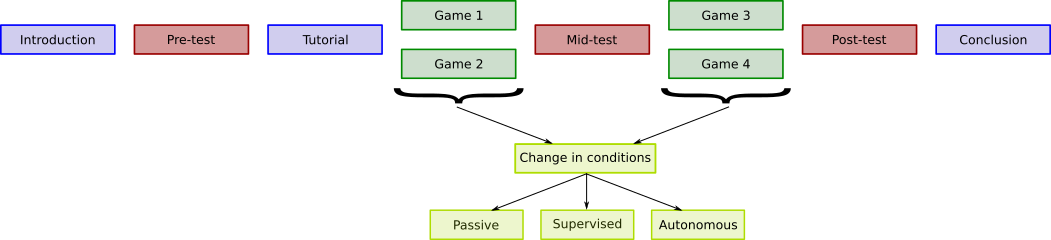
\includegraphics[width=.9\linewidth]{graph.png}
%	\centering
%	\caption{Methodology used for the study.}
%	\label{fig:method}
%\end{figure}

\subsection{Conditions}
The study evaluated three conditions: the passive condition, supervised condition and autonomous condition. In all the conditions, the robot's behaviour during the introduction, tests, tutorial and conclusion was identical. The only change of behaviour happened during the games sessions. The study design was between participants, so children were each assigned to a condition, and in all the game session, the robot would be always the same, passive, supervised or autonomous. %In the passive condition, the robot does not provide support during the game. In the supervised condition, the robot is controlled by a PhD student in psychology acting as the robot's teacher and demonstrating it how to interact. And in the autonomous condition, the robot simply applies the learned policy without supervision.

\subsubsection{Passive Condition}

The \textit{passive} condition served as a control condition. We decided to use a robot even in the control condition to prevent confounds related to the presence of a robot, such as novelty effect. The goal of the study is not to explore if a robot can be better than a human or than just the sandtray, but to study if by using \gls{sparc}, a human can teach the robot a behaviour having a positive influence on the children in the game. In this passive condition, the robot did not provide any advice nor feedback to the children during the game sessions, it only oscillated slightly to simulate a breathing motion and followed the child's face. 


%In the \textit{supervised} condition, the robot was remotely supervised by an operator using \gls{sparc}. Finally, in the \textit{autonomous} condition, the robot applied the learnt policy and provided feedback and guidance to the child without human supervision.


\subsubsection{Supervised Condition}

The \textit{supervised} condition was the one in which the robot learned, the one where \gls{sparc} was used by a human teacher to teach the robot an efficient action policy. As such, it is not a static condition with an identical behaviour all the way, but a dynamic condition where the robot learns an action policy through the human supervision, while the teacher herself is evolving, getting used to controlling the robot. In theory, throughout the different interactions with the children, the behaviour expressed by the robot with the children should be similar and constantly appropriate. In contrast, during that time, the teaching interaction, between the teacher and the robot should evolve due to the learning component on the robot side. 

\subsubsection{Autonomous Condition}

The \textit{autonomous} condition was used to evaluate if the learned behaviour was efficient and if the robot could display a useful social action policy without being supervised. During this condition, the robot used the action policy taught in the supervised condition, but without the teacher in the action selection loop. As such, this condition had to be ran after the supervised one, when the teaching was over. %The role of this condition is to evaluate if the robot did learn a useful action policy, i.e. explore if after having been taught, the robot can have an autonomous behaviour having a positive impact on the child experience.

In the autonomous condition, the robot used the suggestions from the algorithm and executed them with a probabilistic delay between 0 and 1.5 seconds based on the teacher's delay in answering the robot's propositions. This delay aimed to give a pace and synchronisation of actions similar to the ones exhibited by the teacher when reacting to the robot's suggestion.

\subsection{Teacher}
In the study, the teacher was a psychology PhD student from the university, with limited knowledge in computing and machine learning. She had been instructed how to control the robot using the GUI, the effect of each buttons and how to perform each action. She was knowledgeable of the methodology used to run the study (but not the underlying implementation) and experimented controlling the robot in two interactions with the author interacting with the robot and one with a child before starting to supervise the robot for the supervised condition. No information about the learning algorithm or the representation of the state and no feedback about optimal way of interacting or feedback on her action policy was provided before or during the supervision. As such, this robot teacher represents typical target populations for robotic applications: non-experts in machine learning or computing but with relevant domain knowledge such as teachers, psychologists or more broadly, people from the general population.

% Figure~\ref{fig:tutoring_game} shows an example of the game screen. The child can move 10 animals across the game field and can have them interact with other animals or plants. Animals lose energy over time and by interacting with their food the can regain some. Animals that are eaten lose a chunk of their life. The goal for the children is to keep animals alive as long as possible by feeding them and they earn stars representing how healthy their animals have been during the session. The game stops when 3 or more animals run out of energy and each game session lasted 1.6 minutes in average.

\subsection{Metrics}

%Redundant with hypothese?
%This study aimed mostly at evaluating if \gls{sparc} allows a human non-expert in computing to teach a robot from in-situ supervision. 
%This teaching capability is divided into three parts: 
%\begin{itemize}
%	\item How similar the teacher's and autonomous robot's policies are? 
%	\item What are the impacts of the active robot on the child behaviour? \\(And what are the differences between the autonomous and supervised robots?)
%	\item How the online learning component changed the interaction between the robot and the teacher?
%\end{itemize}

To address the hypotheses presented in Section~\ref{sec:tutoring_scope}, we collected multiple metrics on both interactions (teaching and application). First, we recorded the actions executed by the robot in the supervised and autonomous conditions to characterise the two action policies. Two groups of metrics have been collected to evaluate the application interaction: the learning metrics (corresponding to the children's performance during the test) and the game metrics (corresponding to the children's behaviour during the game). And finally, in the supervised condition, we recorded the origin of the action executed by the robot (teacher vs algorithm) and the outcome of the proposed actions (executed vs refused).

\subsubsection{Policy Characterisation}

During the game, the robot had access to 655 actions, which can be divided in seven categories: drawing attention, moving close, moving away, moving to, congatulation, encouragements and reminding rules. Due to this high number of actions, the largeness of the state space (210 dimension) and the complex interdependence between actions and states, totally defining a policy is impossible. Consequently, we decided to use the number of actions executed for each category per child to characterise the policy executed by the robot in the active conditions (supervised and autonomous). While not perfectly representing the action policy of each condition (e.g. the timing of actions is missing), this metric offers a proxy to compare these policies. 

\subsubsection{Learning Evaluation}
The learning was evaluated through an open graph where children had to connect animals to their food. Figure~\ref{fig:test} shows two examples of the test, with or without all the correct connections. Children were instructed to connect as many animals as possible. During the pre-test, the experimenter demonstrated how to connect animals by drawing an arrow from the frog to the fly, and then removing the arrow by pressing the \textit{X} button. When children thought they were done, they could press the `Continue' button, showing a screen asking confirmation to quit the test or allowing children to keep connecting animals. Additionally, the robot informed the child if not all the animals were connected to a food or that animals could eat many types of food if no more than one animal was connected to two items. 

\begin{figure*}[ht]
	\centering
	\begin{subfigure}[t]{0.5\textwidth}
		\centering
		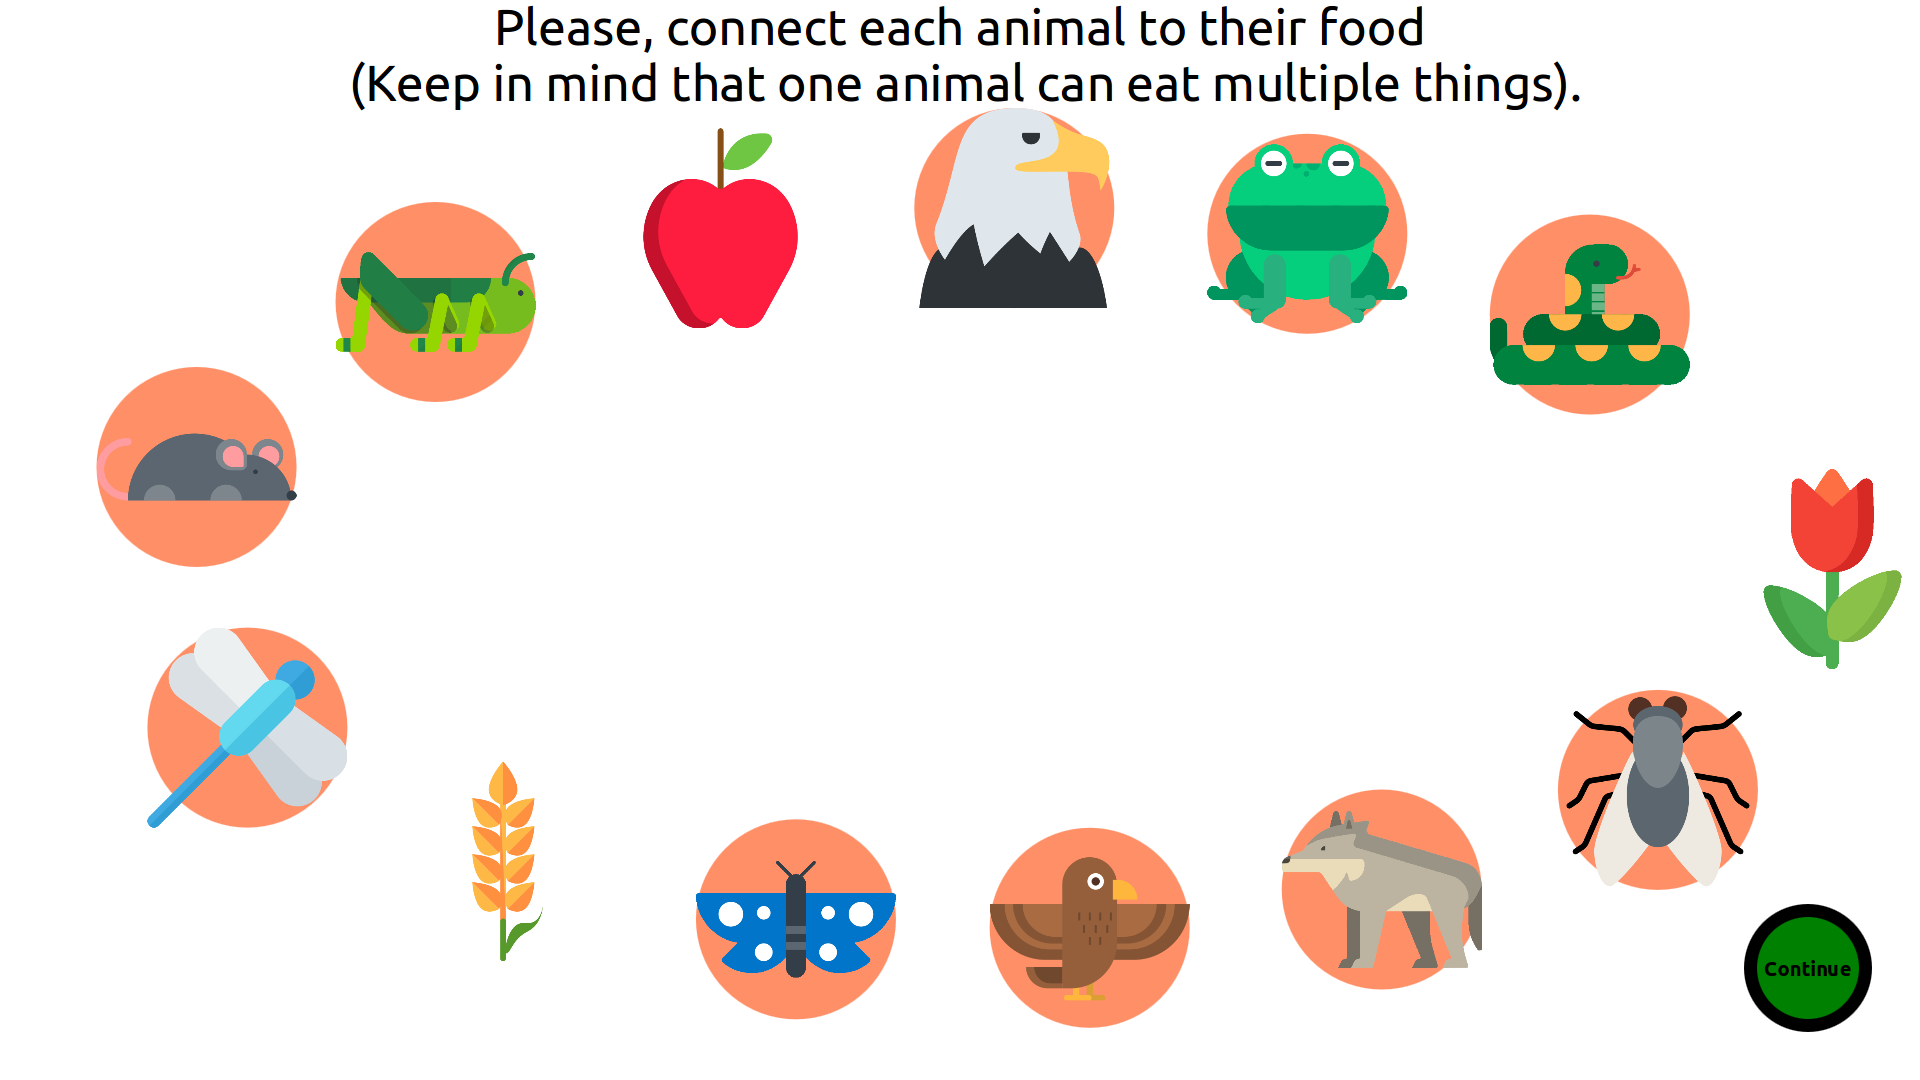
\includegraphics[width=0.95\textwidth]{empty_graph.png}
		\captionsetup{width=.95\linewidth}
		\caption{Empty screen that children face at each test. Red dots behind animals indicate that they are not connected to any food.}
	\end{subfigure}%
	~ 
	\begin{subfigure}[t]{0.5\textwidth}
		\centering
		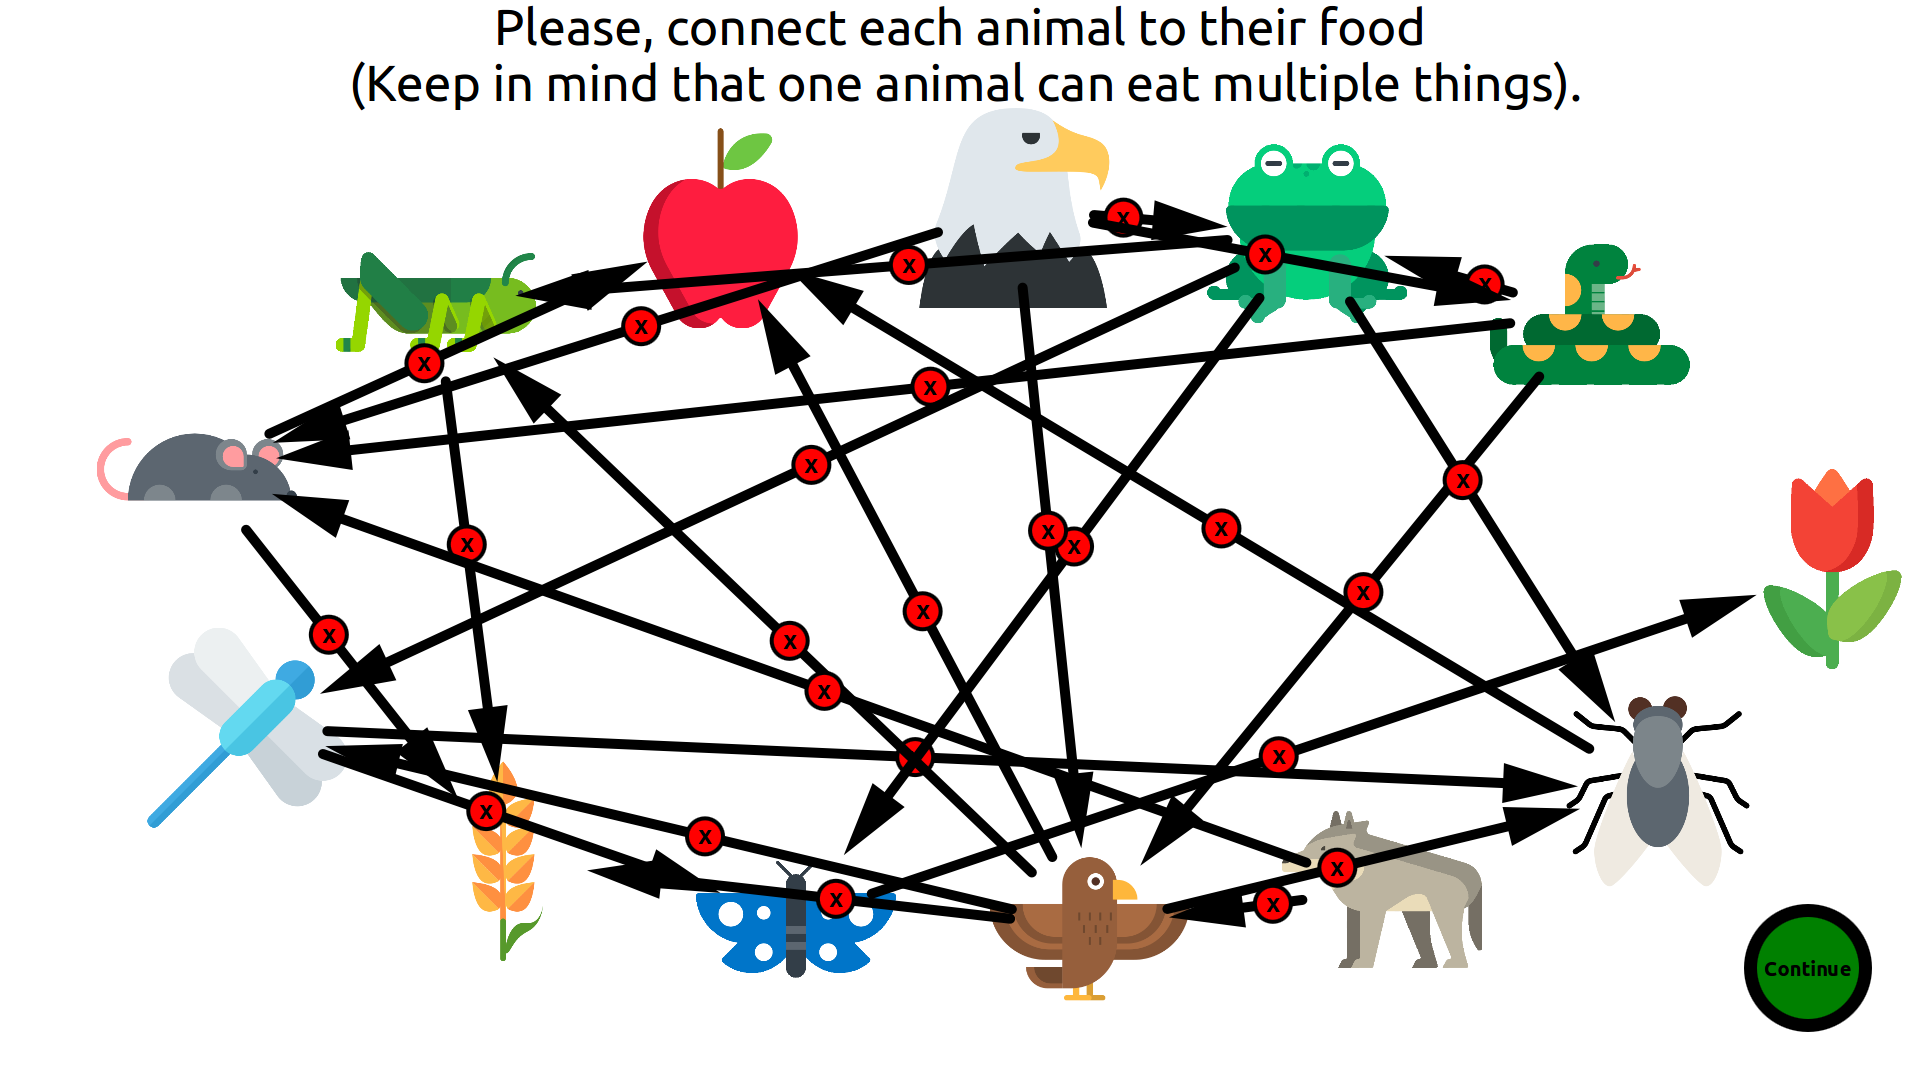
\includegraphics[width=0.95\textwidth]{full_graph.png}
		\captionsetup{width=.95\linewidth}
		\caption{Fully connected test with all the correct connections.}
	\end{subfigure}
	\caption{Test screen to evaluate children's knowledge, empty starting screen (a) and fully connected and correct test (b).}
	\label{fig:test}
\end{figure*}

They are in total 25 different correct connections and 95 possible incorrect ones. As the child can connect as many arrows as desired, the performance is defined as the number of correct arrows above chance (for the number of connected arrows on the test) divided by the maximum achievable performance to reach a score bounded to $[-1,1]$. For example, if a child connects 5 good arrows and 3 bad, their performance would be:

\begin{equation}
P=\frac{\#good-(\#good+\#bad) \cdot \frac{total good}{total}}{total good - total good \cdot \frac{total good}{total}} = \frac{5-(5+3) \cdot \frac{25}{25+95}}{25 - 25 \cdot \frac{25}{25+95}}=0.168
\end{equation}
			
The three tests (pre, mid and post interaction) result in three performance measures. To account with initial differences of knowledge and the progressive difficulty to gain additional knowledge, we computed the learning gain as the difference between the final and initial knowledge divided by the `progression margin': the difference between the maximum achievable performance and the initial performance. This learning gain indicates how much of the missing knowledge the child managed to gain from the game.
			
\subsubsection{Game Metrics}
Different metrics have been gathered during the game sessions to characterise the children's behaviours:
\begin{itemize}
	\item \textbf{Number of different eating interactions}: number of unique feeding action type [0,25].
	\item \textbf{Points}: cumulated sum of animals' energy over the game (typical range [550,1100]).
	\item \textbf{Interaction time}: Duration of game sessions, how long a game lasted until three animals ran out of energy (typical range [.5,3] minutes).
\end{itemize}

The number of different eating interactions informs on how many learning items the children have encountered in the games. A feeding interaction happens when an animal is moved to its food (or to a predator); and the number of different feeding interaction represents how many different unique correct connections the child been exposed to during the game (multiple feeding actions between the same animals would count only once). A game with a high number of different feeding represents a game where the child had the opportunity to learn many correct connections between animals. Consequently, by increasing this number, the children would be exposed to more learning items which should help them to perform better on the tests. Both the interaction time and the number of points reached in the game inform on the children's success in the task: keeping the animals alive as long as possible. 

%Maybe talk about compliance

\subsubsection{Robot Learning}

In the supervised condition, the robot executed actions selected or validated by the teacher, and by using \gls{sparc}, the robot could propose actions to the teacher. Faced with a proposition, the teacher had multiple ways to react. They could accept the action (by waiting for it to be executed, pressing `Do it' or selecting the same action manually) or refuse it (by pressing the `Cancel', `Skip' or `Remove' buttons). As such, actions going through this pipeline can be divided in three categories: actions selected by the supervisor, robot's good propositions and robot's bad propositions. And the evolution of these categories represents how much the online component of the learning improved the quality of the robot's suggestions and reduced the workload on the teacher. 

Some times the teacher cancelled actions and then selected them again, we called this effect the `reselection'. To obtain the final numbers of accepted and refused actions, we removed these reselection from the bad propositions and we added them to the good propositions as it represents cases where the teacher refused an action by accident.

\section{Results}

% and right graphs present the 

%Preliminary results (currently in progress, due to be completed before the submission of the full article) show that (1) the robot is able to effectively jointly learn action and social policies (Figure 2), (2) the learning gains of the children supported by the autonomous robot are not significantly different from the gains when the learning is supported by a robot teleoperated by the human expert, which would indicate the utility of the approach.

Similarly to Chapter~\ref{chap:control}, we analysed the results using Bayesian statistics and the JASP software~\citep{jasp2018}. We used a Bayesian mixed ANOVA as omnibus test to explore the impact of conditions or repetition on the metrics. Additional post-hoc tests use a Bayesian mixed ANOVA comparing the conditions one by one and fix the prior probability to 0.5  to correct for multiple testing.

\subsection{Example of a Session}
\ES{Probably not the best, but I can check}

Table~\ref{tab:tuto_session} presents an example of the first 50 seconds of a session. Propositions from the robot are in blue, and actions from the teacher in orange. It should be noted that in some cases, the teacher did not evaluate actions proposed by robot, but just selected an other action. In that case, the action proposed is not evaluated and the selected action is executed and stored in memory.

\begin{table}[ht]
	\centering
	\ra{1}
	\caption{Example of events during the first 50 seconds of a session.}
	\label{tab:tuto_session}
	\begin{tabularx}{\textwidth}{@{}L{.2}L{1.8}|L{.2}L{1.8}@{}}\toprule
		Time & Event & Time & Event\\
		\midrule
4.1 & childtouch frog & 27.7 & childtouch fly\\
4.3 & failinteraction frog wheat-3 & 28.0 & childrelease fly\\
4.9 & animaleats frog fly & 28.4 & childtouch dragonfly\\
5.8 & childrelease frog & 28.6 & failinteraction dragonfly apple-1\\
6.6 & \textcolor{SkyBlue}{robot proposes congrats} & 29.1 & childrelease dragonfly\\
7.6 & childtouch fly & 29.4 & failinteraction dragonfly apple-1\\
7.6 & \textcolor{BurntOrange}{teacher selects wait} & 30.3 & childtouch dragonfly\\
8.0 & animaleats fly apple-4 & 30.3 & failinteraction dragonfly apple-1\\
8.3 & childrelease fly & 30.7 & \textcolor{SkyBlue}{robot proposes encouragement}\\
9.1 & \textcolor{BurntOrange}{teacher selects congrats} & 31.0 & failinteraction dragonfly apple-1\\
9.1 & childtouch frog & 31.8 & \textcolor{BurntOrange}{teacher selects wait}\\
10.3 & childrelease frog & 32.5 & childrelease dragonfly\\
10.8 & childtouch frog & 34.4 & childtouch wolf\\
11.2 & animaleats frog fly & 34.7 & \textcolor{SkyBlue}{robot proposes remind rules}\\
12.4 & failinteraction frog apple-2 & 35.0 & animaleats wolf mouse\\
12.5 & animaleats frog fly & 36.0 & \textcolor{BurntOrange}{teacher selects wait}\\
13.2 & childrelease frog & 36.0 & animaleats wolf mouse\\
14.2 & childtouch fly & 37.2 & childrelease wolf\\
14.5 & animaleats fly apple-2 & 37.7 & childtouch grasshopper\\
14.6 & \textcolor{SkyBlue}{robot proposes encouragement} & 38.3 & \textcolor{SkyBlue}{robot proposes congrats}\\
15.0 & childrelease fly & 41.8 & reset\\
15.4 & animaleats fly apple-3 & 42.1 & failinteraction grasshopper apple-1\\
16.9 & \textcolor{BurntOrange}{teacher selects encouragement} & 42.7 & childrelease grasshopper\\
18.2 & childtouch snake & 42.7 & failinteraction grasshopper apple-1\\
18.4 & failinteraction snake wheat-3 & 44.4 & \textcolor{BurntOrange}{teacher selects mvc mouse wheat-1}\\
18.7 & animaleats snake bird & 44.6 & robottouch mouse\\
19.6 & animaleats snake bird & 44.7 & childtouch butterfly\\
20.5 & childrelease snake & 45.1 & failinteraction butterfly wheat-2\\
20.6 & failinteraction snake wheat-4 & 45.6 & childrelease wheat-1\\
20.6 & \textcolor{SkyBlue}{robot proposes congrats} & 45.6 & robotrelease mouse\\
20.9 & childtouch eagle & 45.7 & robottouch mouse\\
21.1 & animaleats eagle bird & 48.9 & robotrelease mouse\\
22.0 & animaleats eagle bird & 49.3 & childtouch butterfly\\
22.4 & childrelease eagle & 49.3 & failinteraction butterfly wheat-1\\
23.3 & animaldead bird & 49.6 & childrelease butterfly\\
23.4 & \textcolor{BurntOrange}{teacher selects mvc dragonfly fly} & 50.0 & childtouch mouse\\
23.6 & robottouch dragonfly & 50.3 & animaleats mouse wheat-1\\
26.9 & robotrelease dragonfly & 51.0 & childrelease mouse\\
		\bottomrule
	\end{tabularx}
\end{table}

\subsection{Comparison of Policy}

Figure~\ref{fig:tutoring_actions_distribution} presents the number of actions of each types executed by the teacher (in the supervised condition) and the autonomous robot. Both action policies presented similarities: the action `Move away' was almost never used, `Move to' was never used, and the supportive feedback (`Congratulation' and `Encouragement') were used more often than `Remind rules' or `Drawing attention'. However, some dissimilarities were also present, for instance, the autonomous robot used more encouragements than congratulations while the teacher did the opposite. The autonomous robot also reminded the rules more often and used the `Move close' action less than the supervisor. These differences of actions are probably linked to the type of machine learning used; with instance based learning, some datapoints will be used in the action selection much more often than others, which might explain these biases. But these results show that the robot managed to learn a social and technical action policy presenting similarities with the one displayed by the teacher providing partial support for H1.

\begin{figure}[ht]
	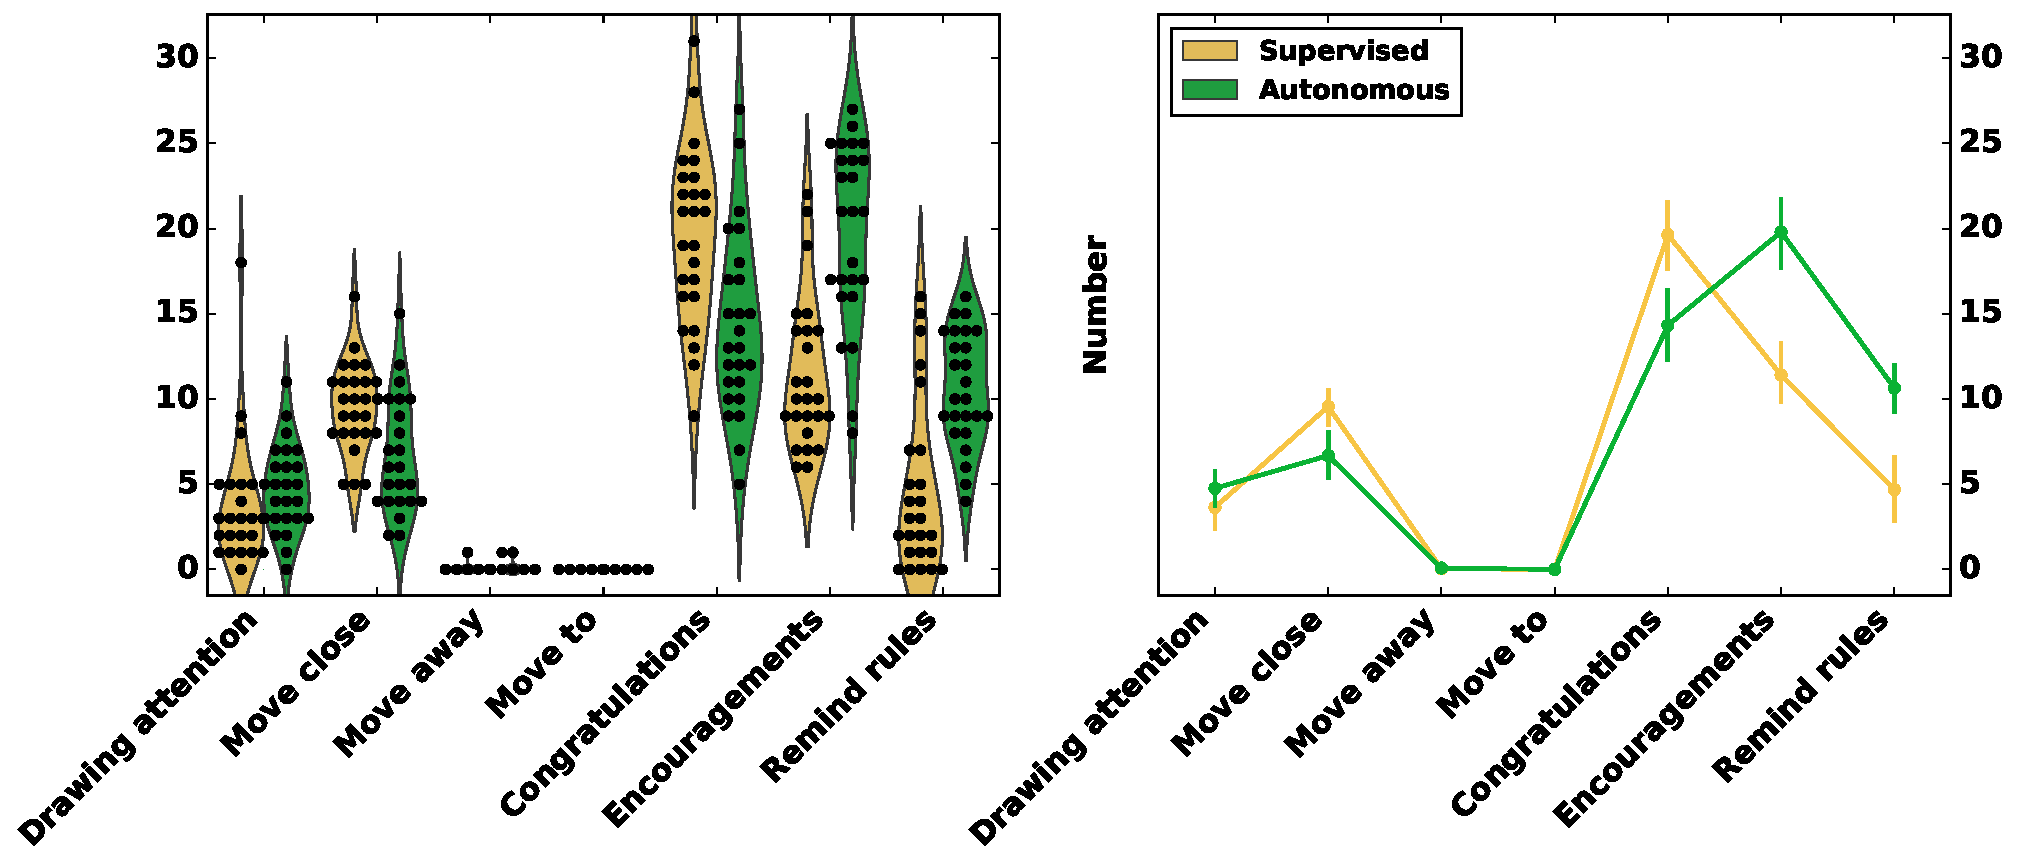
\includegraphics[width=1\linewidth]{actions.pdf}
	\centering
	\caption{Comparison of actions executed for the autonomous and supervised condition. The left graph is a violin plot of the data, while the right presents the means and the 95\% Confidence Intervals}
	\label{fig:tutoring_actions_distribution}
\end{figure}


%\begin{figure}[ht]
%	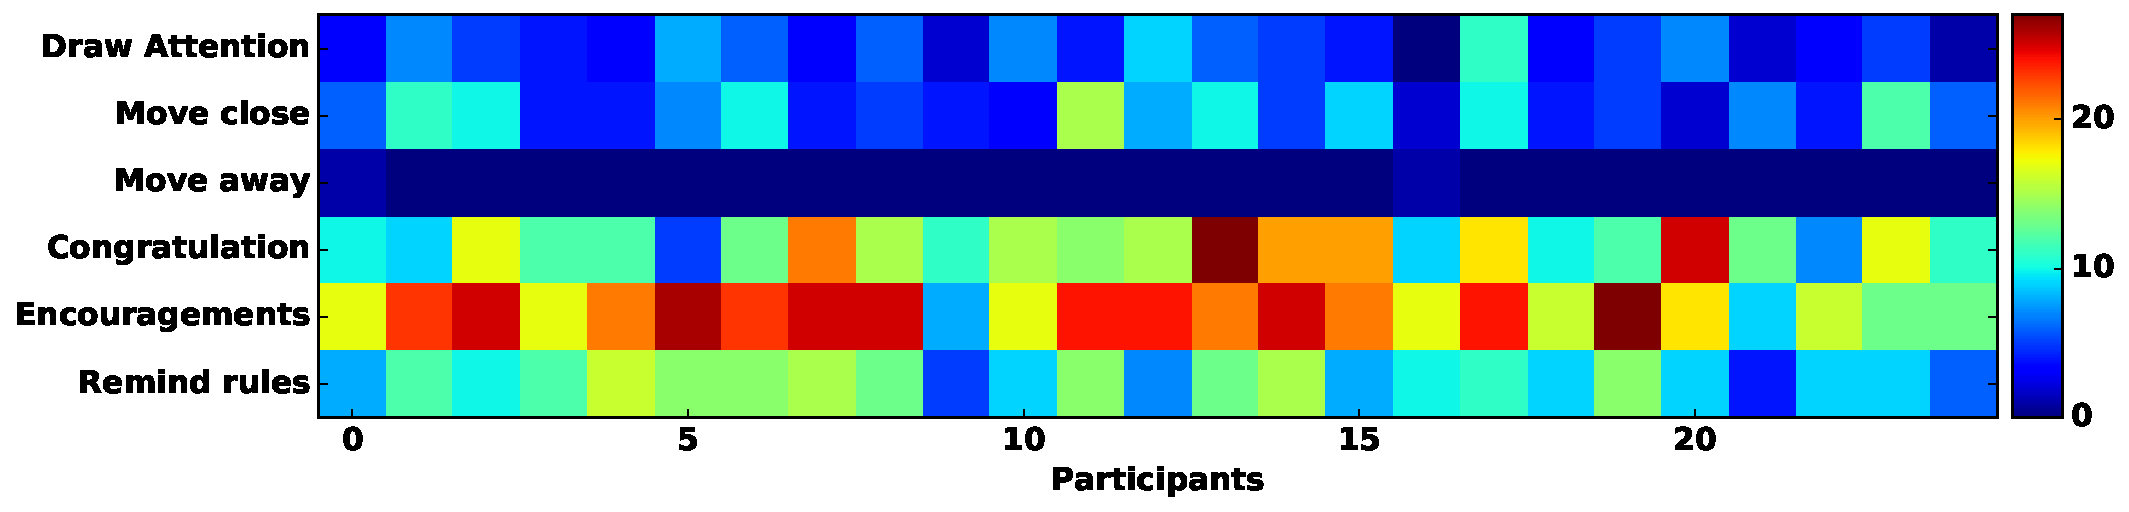
\includegraphics[width=1\linewidth]{autonomous_actions.pdf}
%	\centering
%	\caption{Repartition of actions across the participants in the autonomous condition.}
%	\label{fig:tutoring_autonomous_actions}
%\end{figure}
%
%\begin{table}[ht]
%	\centering
%	\caption{Repartition of action in the policy for both conditions (in \%).}
%	\label{tab:tutoring_policies}
%	\begin{tabularx}{\textwidth}{@{}lYYYccY}\toprule
%		& Draw \newline Attention & Move \newline close & Move \newline away & Congratulation & Encouragements & Remind \newline rules \\
%		\midrule
%		Supervised & 6.6  & 22.2 & 0.1 & 43.1 & 22.7 & 5.3 \\
%		Autonomous & 8.5 & 11.8 & 0.1 & 25.4 & 35.2 & 18.9\\
%		\bottomrule
%	\end{tabularx}
%\end{table}


\subsection{Test Performance}

Figure~\ref{fig:tutoring_performance} shows the evolution of children's performance across the three tests. A Bayesian mixed-ANOVA showed that in all conditions, children's performance increased across the tests ($B=1.5$x$10^{12}$), however the impact of the condition on the learning was inconclusive with a tendency to show no impact ($B=0.539$). This indicates that by being involved in the task, every children learned and improved their performances on the test (by gaining in average 13\% of the missing knowledge), but the robot behaviour during the game did not have an important impact on the children's learning gain (see Figure~\ref{fig:tutoring_learning}), invalidating H2.

\begin{figure}[ht]
	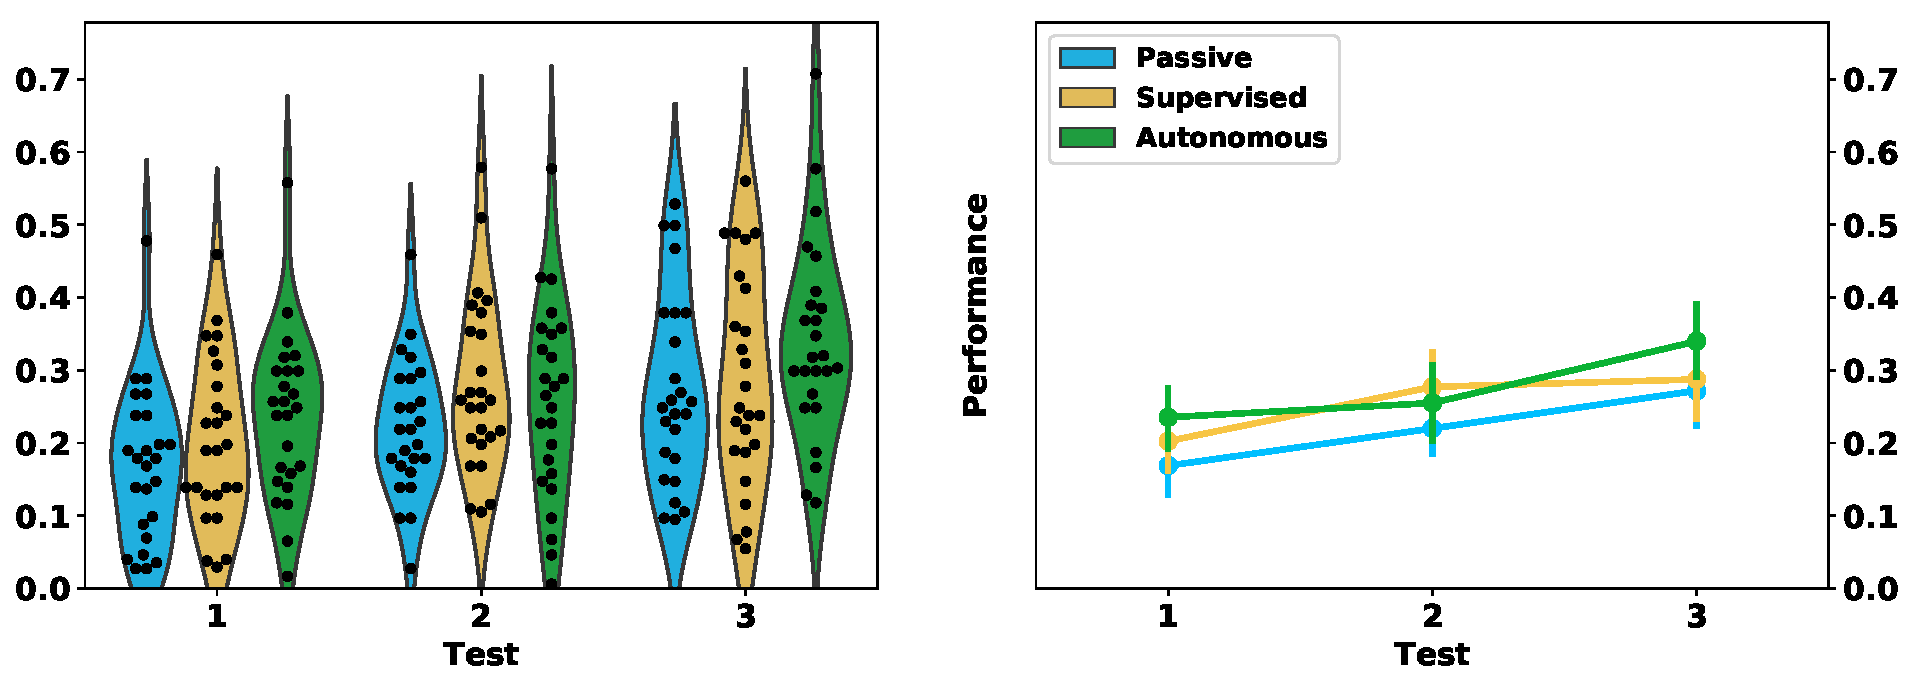
\includegraphics[width=1\linewidth]{perf.pdf}
	\centering
	\caption{Children's performance for the three tests: pretest, midtest and posttest for the three conditions.}
	\label{fig:tutoring_performance}
\end{figure}

\begin{figure}[ht]
	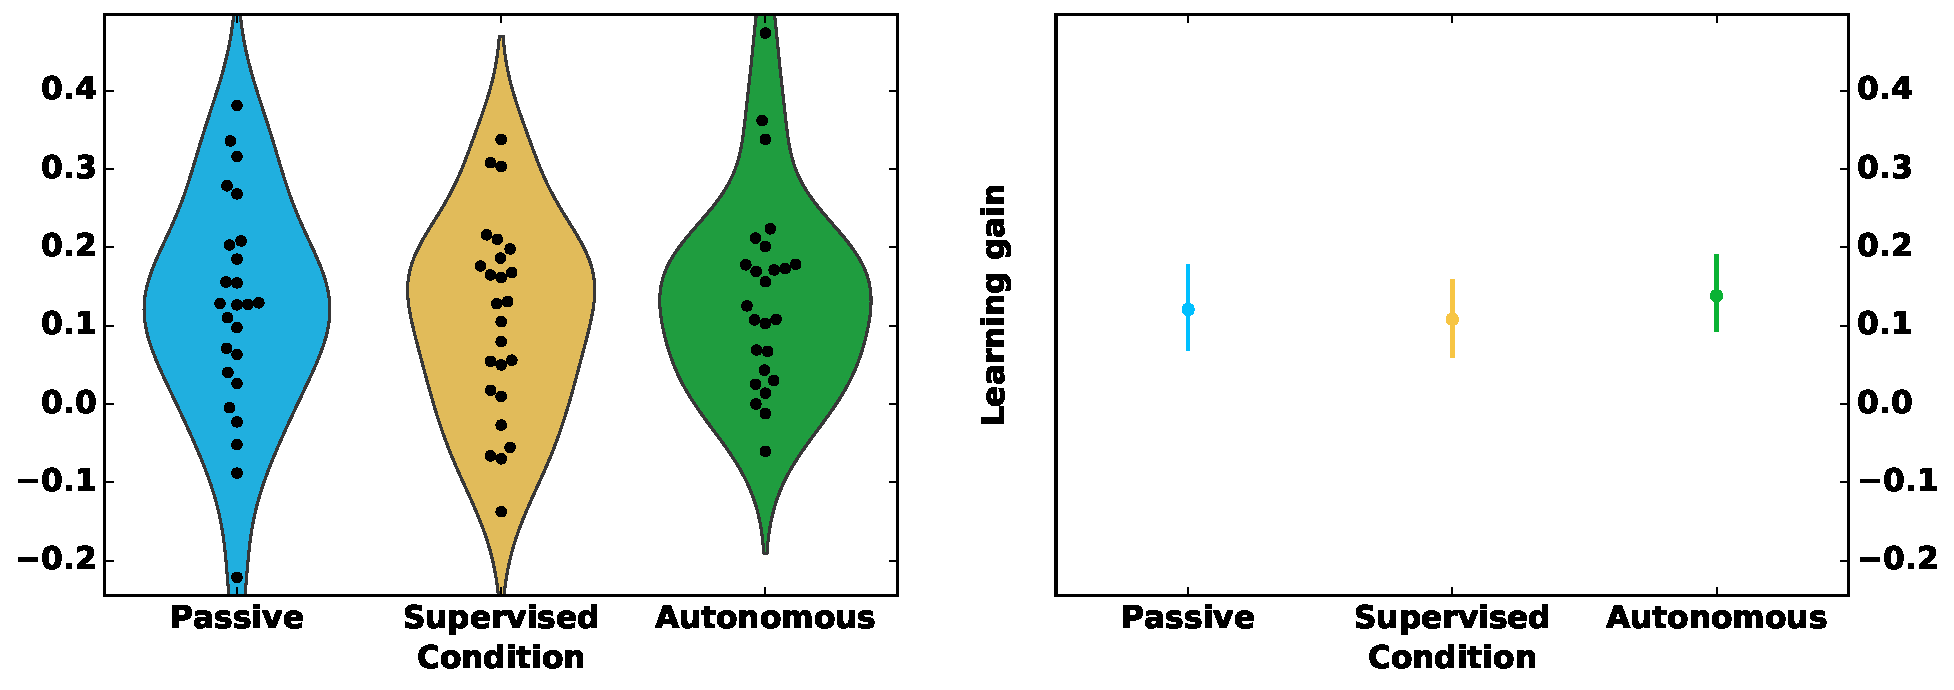
\includegraphics[width=1\linewidth]{learning.pdf}
	\centering
	\caption{Children's normalised learning gain after interacting with the robot for the three conditions.}
	\label{fig:tutoring_learning}
\end{figure}

\subsection{Game Metrics}

\paragraph{Different eating behaviours}
Figure~\ref{fig:tutoring_d_eat} shows the evolution of the number of different eating behaviours exhibited by the children across the four game sessions. A Bayesian mixed-ANOVA showed an impact of the condition on the number of different eating behaviours produced by the children in the game ($B=6.1$). Post-hoc tests showed the absence of difference between the supervised and the autonomous conditions ($B=0.154$), whilst differences were observed between the supervised and the passive condition ($B=512$) and between the autonomous and the passive conditions ($B=246$). This indicates that, compared to the passive robot, the supervised robot provided additional knowledge to the child during the game, allowing them to create more useful interactions between animals and their food, receiving more information from the game potentially helping them to learn. And the autonomous robot managed to recreate autonomously this effect without the presence of a human providing input.

\begin{figure}[ht]
	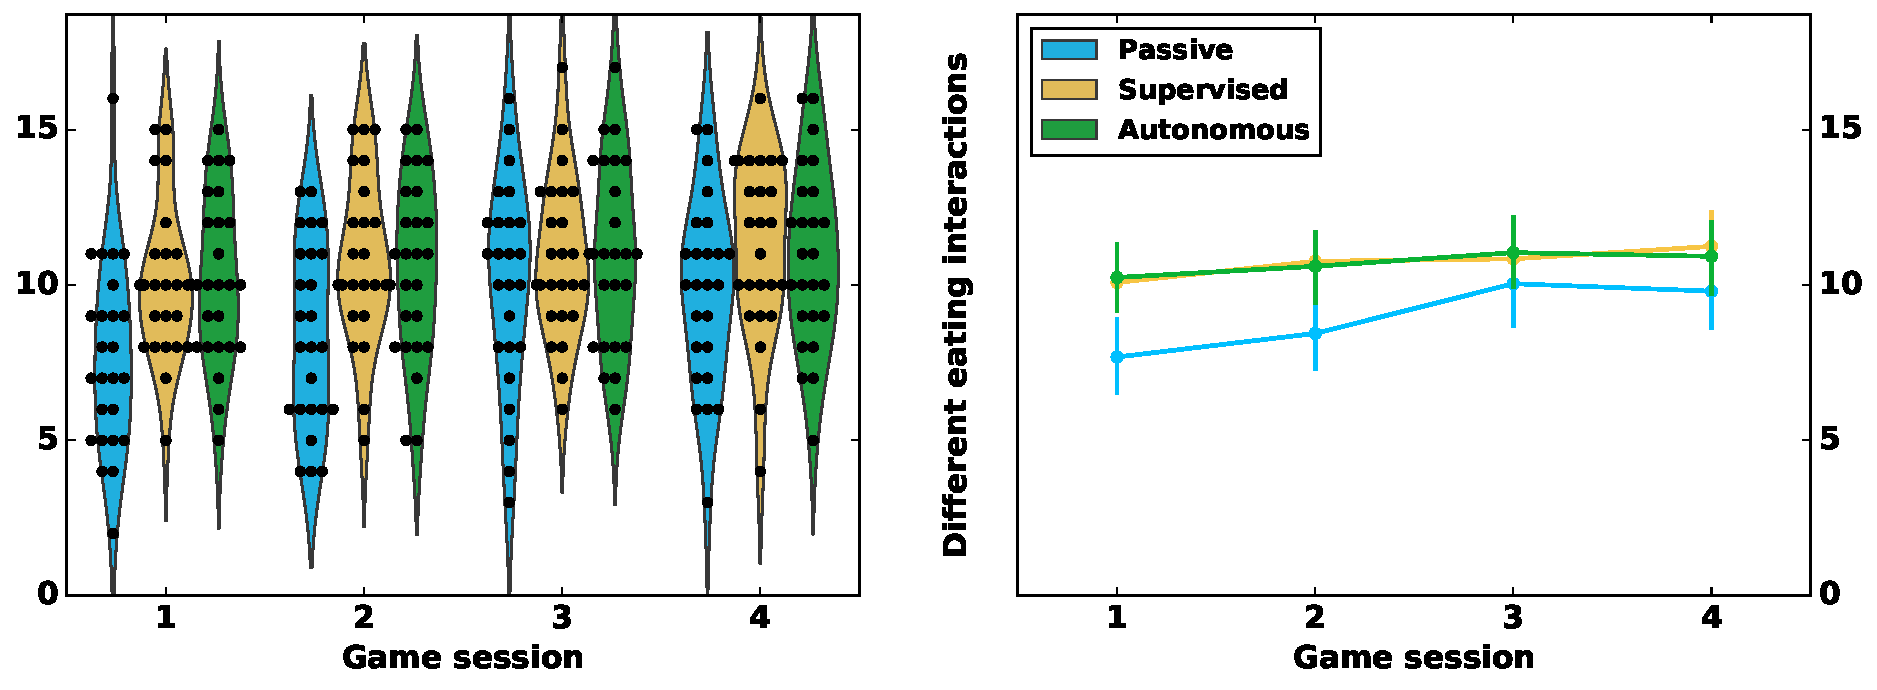
\includegraphics[width=1\linewidth]{d_eat.pdf}
	\centering
	\caption{Number of different eating behaviour for the four games for the three conditions.}
	\label{fig:tutoring_d_eat}
\end{figure}

\paragraph{Points}

Figure~\ref{fig:tutoring_points} shows the evolution of the number of points achieved by the children across the four game sessions. A Bayesian mixed-ANOVA showed an impact of the condition on the number of points achieved by the children in the game ($B=10.2$). Post-hoc tests showed a strong difference between the passive and the supervised conditions ($B=5.1$x$10^4$) and differences between the supervised and the autonomous conditions ($B=5.2$) and the autonomous and the passive condition ($B=5.9$). This indicates that when the robot was supervised, it allowed children to achieve more points than a  passive robot. And a similar effect was observed when the robot is autonomous, however the autonomous robot did not manage to reach the same efficiency as the supervised robot in helping the children to achieve a high score in the game.

\begin{figure}[ht]
	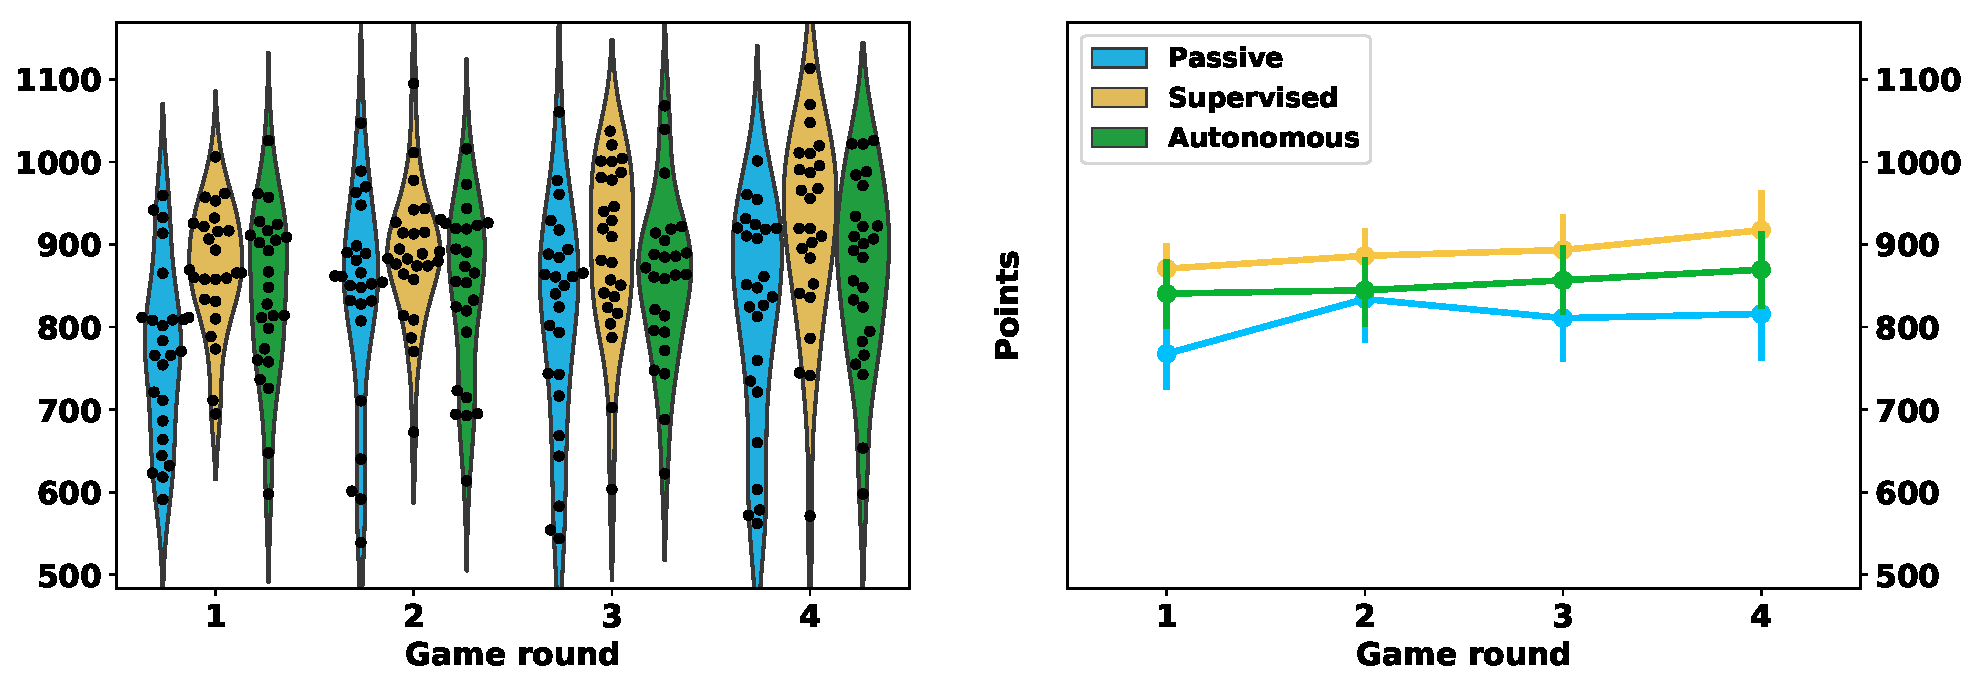
\includegraphics[width=1\linewidth]{points.pdf}
	\centering
	\caption{Points achieved by the children in each game session for the three conditions.}
	\label{fig:tutoring_points}
\end{figure}

\paragraph{Time}

Figure~\ref{fig:tutoring_time} shows the evolution of interaction time across the four game sessions. A Bayesian mixed-ANOVA showed inconclusive results on the impact of the condition on the interaction time in the game ($B=1.1$). However, post-hoc tests showed the absence of difference between the supervised and the autonomous conditions ($B=0.287$), whilst differences are observed between the supervised and the passive condition ($B=118$) and a tendency of difference between the autonomous and the passive conditions ($B=2.9$). This indicates that the supervised robot allowed children to be better at the game, allowing them to maintain animal alive longer than a passive robot. And the autonomous robot learned and applied a policy tending to replicate this effect and without exhibiting differences with the supervised one.

\begin{figure}[ht]
	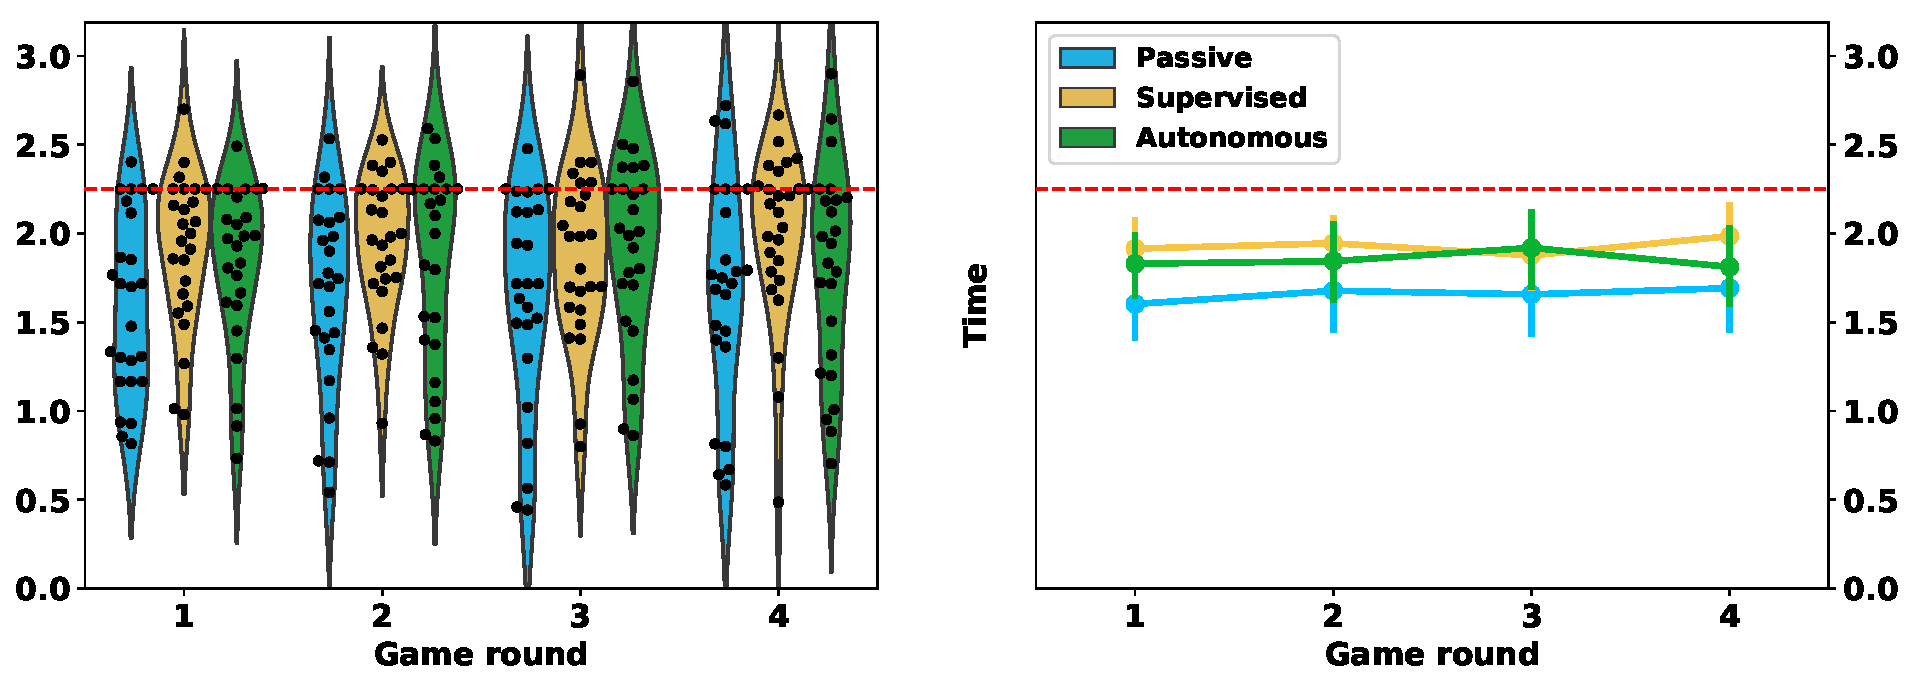
\includegraphics[width=1\linewidth]{time.pdf}
	\centering
	\caption{Interaction time for the four games for the three conditions.}
	\label{fig:tutoring_time}
\end{figure}


\paragraph{Summary}

These game metrics showed that the action policy executed by the autonomous robot allowed children to achieve similar results in the game than when the robot was supervised, and better results than when interacting with a passive robot. This provides support for H1 ("The autonomous robot is able to interact socially and efficiently during the game sessions and maintain the child's engagement during the learning task"). 
%However, children learned similarly in the three conditions, so these improvements in the game did not transfer to improvements in the test neither for the supervised robot nor the Autonomous one. This does not support H1 ("The robot support child learning: learning gain in passive condition $<$ learning gain in autonomous condition $<$ learning gain in supervised condition")

\subsection{Teaching the Robot}

Figure~\ref{fig:tutoring_supervision} presents the reaction of the teacher to the robot's suggestions across all the supervised sessions. In average the teacher accepted 22.3\% of all the proposition of the robot, which represented 35\% of all the actions executed by the robot and this effect tended to be stable across the sessions.

\begin{figure}[ht]
	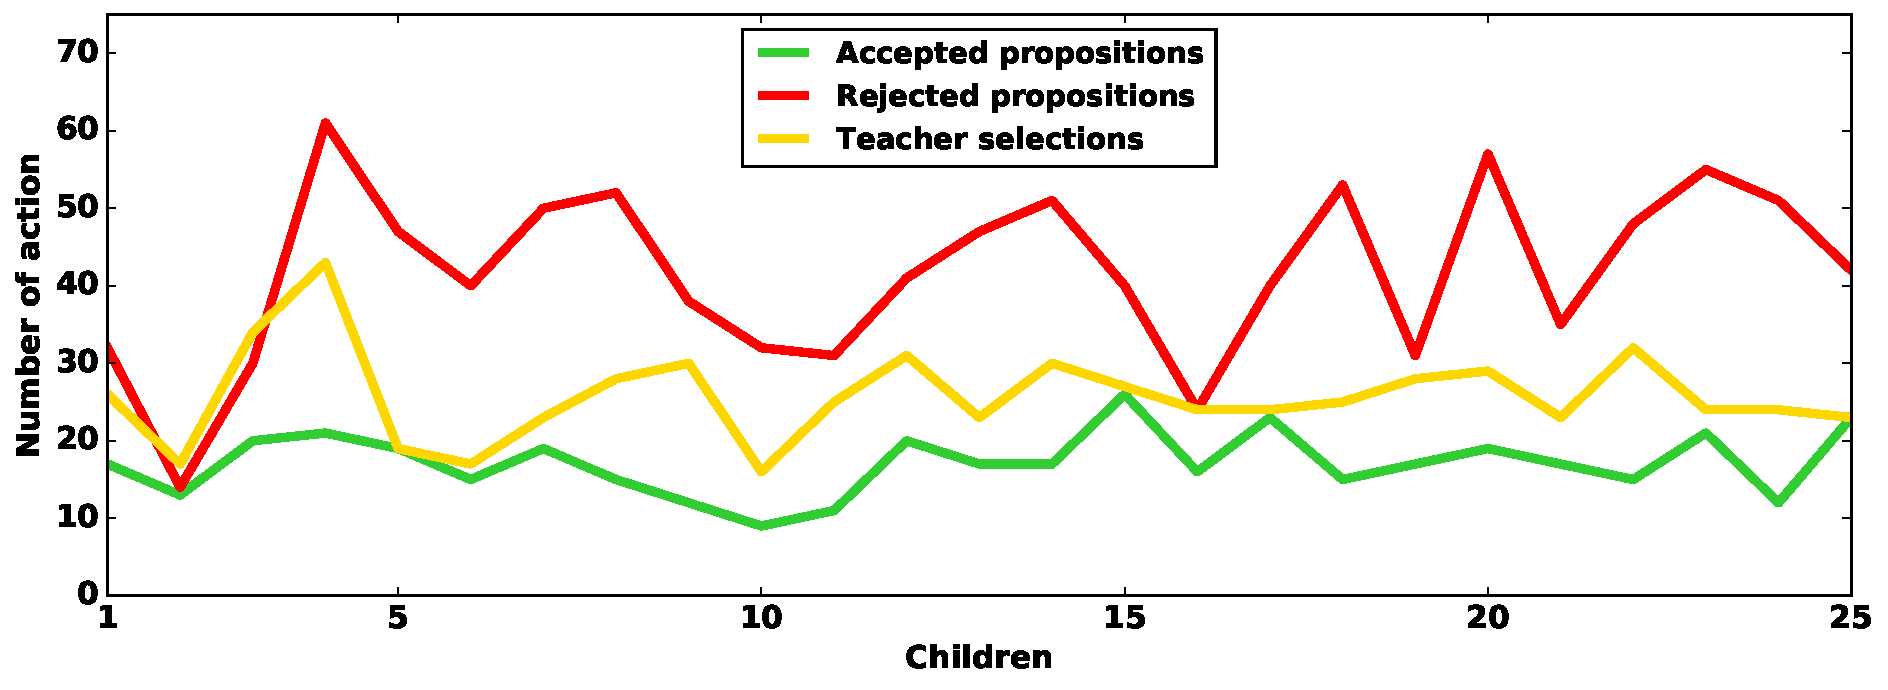
\includegraphics[width=1\linewidth]{./summary_supervision.pdf}
	\centering
	\caption{Summary of the action selection process in the supervised condition: the `teacher selection' label represents each time the teacher manually selected an action not proposed by the robot.}
	\label{fig:tutoring_supervision}
\end{figure}


Figure~\ref{fig:tutoring_actions} presents the accumulated number of different actions in the policy the teacher used. We can observe a sharp increase in the first 5 interactions, when the teacher use the main actions for the first time. Then there is a mixture of small plateau and small increases, indicating that the teacher had phases where she enriched her action policy more. And finally, the number of different actions in the policy seems to converge around 60 toward the last interactions.

\begin{figure}[ht]
	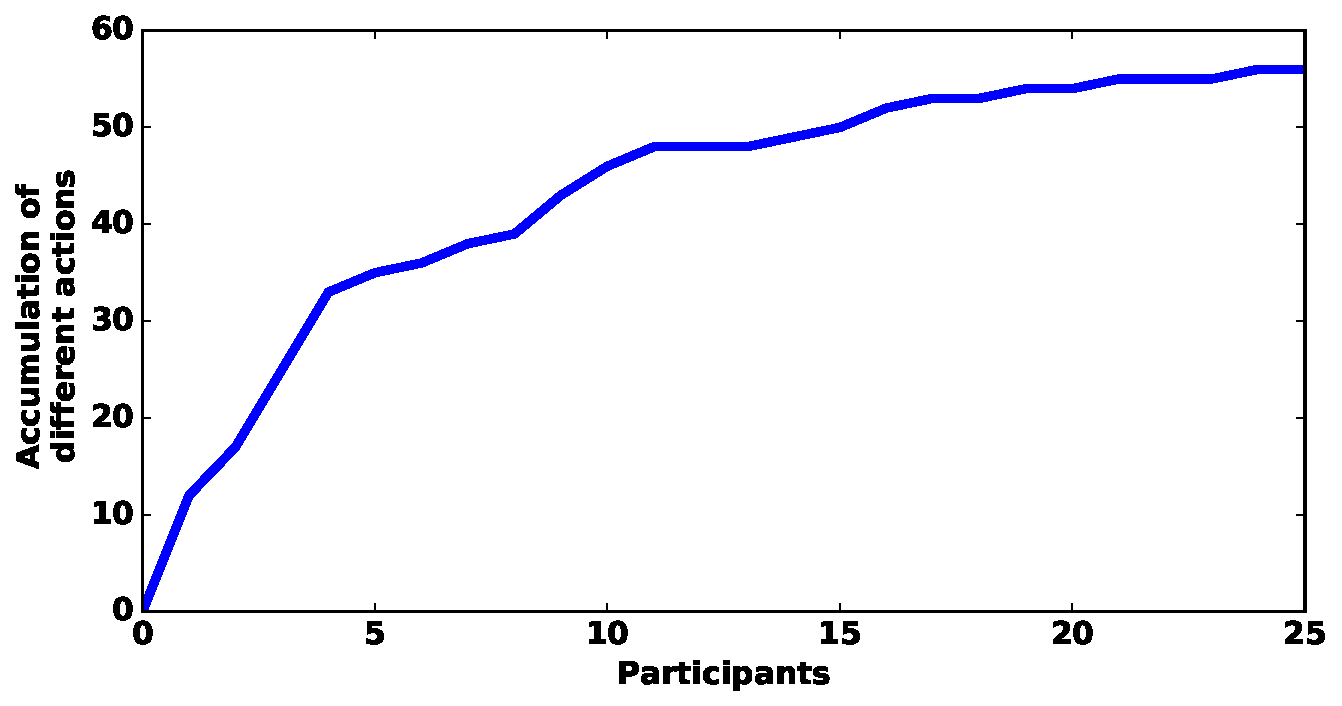
\includegraphics[width=.85\linewidth]{./number_actions.pdf}
	\centering
	\caption{Number of different actions used by the teacher throughout the interactions with the children.}
	\label{fig:tutoring_actions}
\end{figure}


In post-hoc discussion, the teacher reported three phases in her teaching: 
\begin{itemize}
	\item First sessions: she was not paying much attention to the suggestions, mostly trying to have the robot executing a correct action policy.
	\item Session 6 to around 16: she was paying more attention to the suggestions without giving them much credit.
	\item Last sessions: she started to trust the robot more but without ever trusting it totally.
\end{itemize}

%\ES{I should add more about it...}
Appendix~\ref{app:diary} presents a more detailed diary of the teacher throughout her supervision. Additionally, while the buttons cancel and skip has different impact of the learning, and were designed to be used in different cases, the teacher reported that she used them interchangeably.

The teacher did report a decrease of workload as she supervised the robot in more session. This was supported by behaviours such as typing her observations on a laptop, while gazing at the interface in multiple interactions (especially at the start of a session). However this decrease of workload seemed to be due mostly due to the teacher getting used to the interaction, and not to the online learning and the improvement of the suggested proposition, invalidating H3.


%Figure~\ref{fig:tutoring_proposition} presents the reaction of the teacher to the robot's suggestions across all the supervised sessions. In average the teacher accepted 22.3\% of all the proposition of the robot (by enforcing the action, let it be executed or using the `Do it' button), which represents 35\% of the actions executed by the robot. This effect tends to be stable across the sessions. The teacher interaction pattern evolved overtime, such as by using mostly the `Cancel' button in the start then the `Skip' one, but in the end, the teacher used this two buttons mostly interchangeably even if the algorithm underlying reaction is different. Another observation is the evolution from using the auto-execution function to the `Do it' button once the teacher felt more comfortable in the supervision. The teacher reported three phases in her teaching: 
%
%\begin{itemize}
%	\item First sessions: she was not paying much attention to the suggestions, mostly trying to have the robot executing a correct action policy.
%	\item Session 20 to around 65: she was paying more attention to the suggestions without giving them much credit.
%	\item Last sessions: she started to trust the robot more but without ever trusting it totally.
%\end{itemize}
%
%\begin{figure}[ht]
%	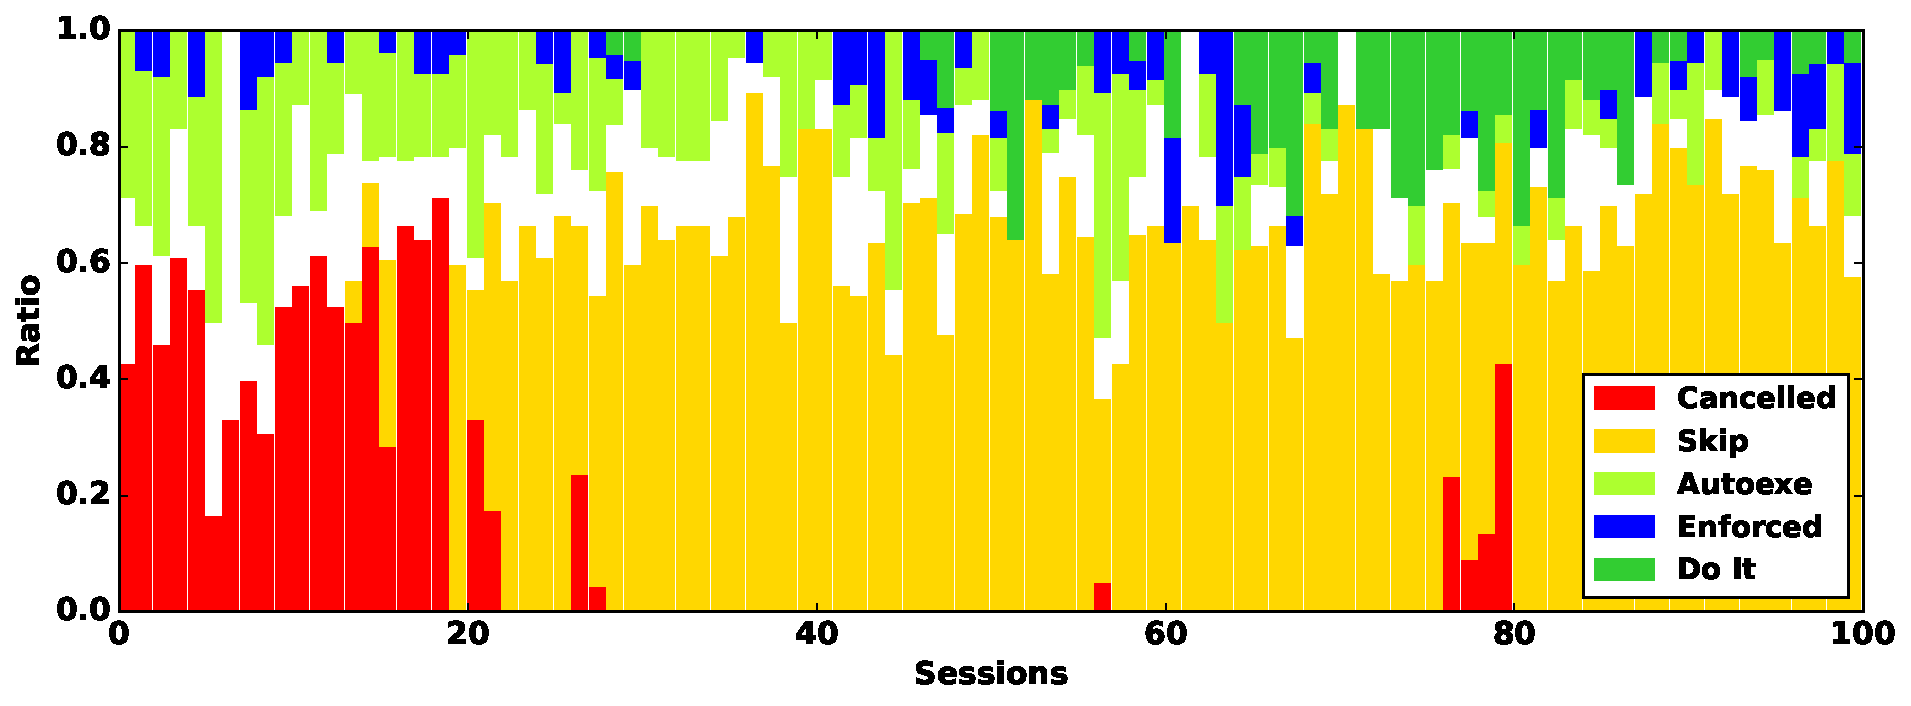
\includegraphics[width=1\linewidth]{propositions.pdf}
%	\centering
%	\caption{Teacher's reaction to the robot's propositions along the sessions.}
%	\label{fig:tutoring_proposition}
%\end{figure}
%
%
%\begin{figure}[ht]
%	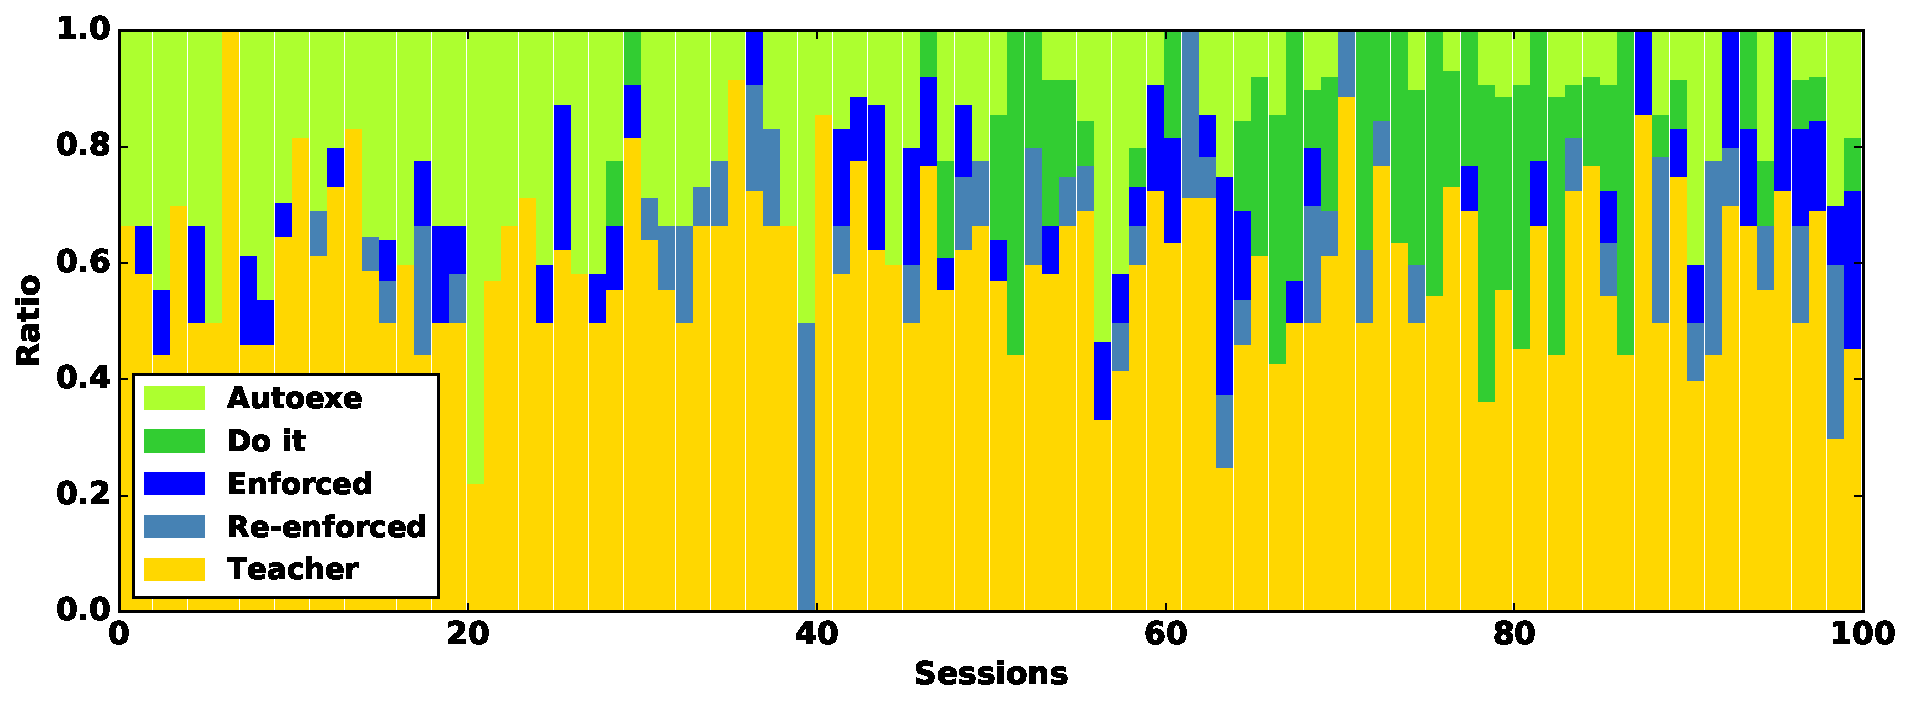
\includegraphics[width=1\linewidth]{selections.pdf}
%	\centering
%	\caption{Origin of the actions executed by the robot. Re-enforced actions indicates that an action has been selected after having been cancelled or skipped by the teacher.}
%	\label{fig:tutoring_selection}
%\end{figure}
%
%Additional comments:
%\begin{itemize}
%	\item The robot proposed in average 58\% more actions than the number of actions selected by the teacher.
%	\item As the time is continue and not discrete, the concept of correct actions is shifted, and actions selected by the teacher might have been proposed by the robot a fraction of second later without being counted as good proposition.
%	\item The teacher often cancelled/skip actions directly as they arrived without taking time to analyse them (limitation of this implementation of SPARC).
%	\item Evolution of teaching policy limits the potential of learning (not one single policy applied by the teacher, but an evolving one).
%	\item Children are different, so the teacher tried to apply different action policy for each child.
%\end{itemize}
%
%
%\begin{figure}[ht]
%	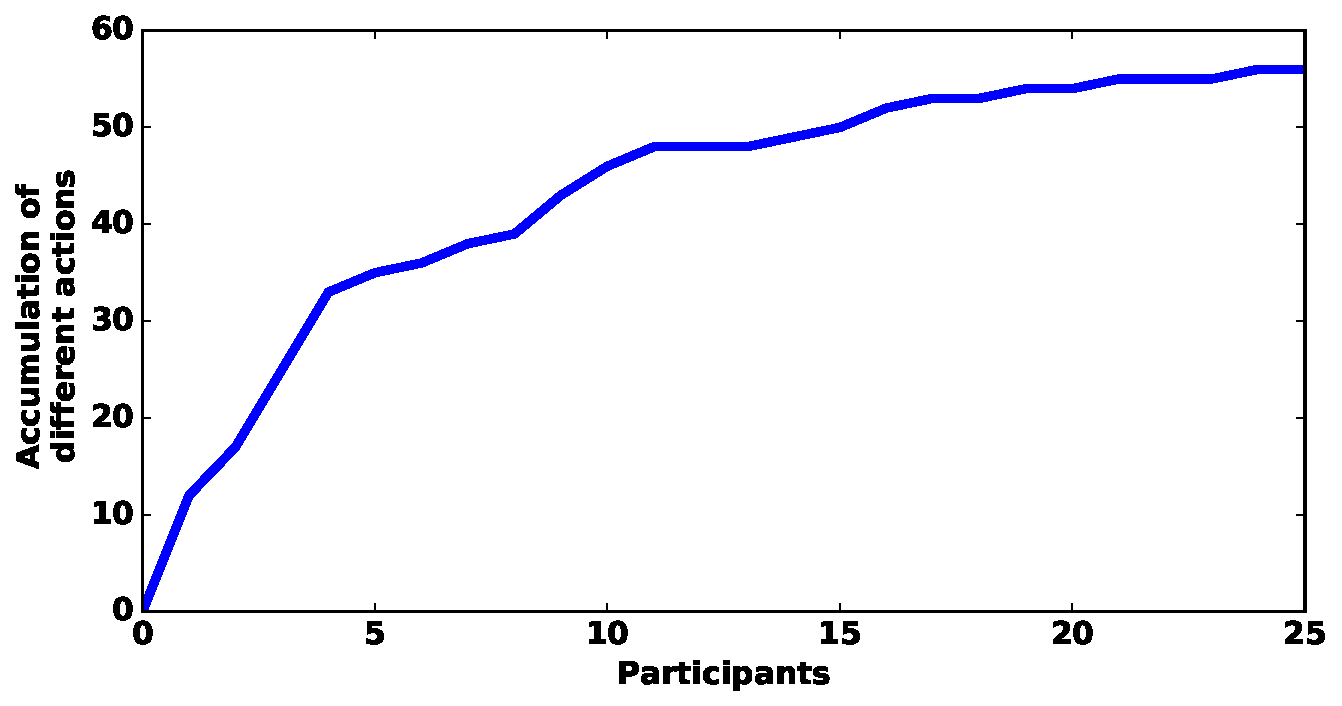
\includegraphics[width=.6\linewidth]{number_actions.pdf}
%	\centering
%	\caption{Accumulation of the number of different actions used by the teacher across the  participants.}
%	\label{fig:tutoring_actions}
%\end{figure}


\section{Discussion} \label{sec:tutoring_discussion}

\subsection{Children Behaviours and Learning Gain}

The active robots' behaviour encouraged children to produce more `useful' behaviours during the interaction. When interacting with the active robots, children encountered more situations with learning potential (such as the different eating behaviours). However, this additional exposure to learning items did not transform into an increase in learning gain. In the three conditions, the children learned similarly; thereby not supporting H2. We identified two possible roots for this absence of transfer between positive game behaviours and performance in the test. The first one is that the game by itself, without the robot, encouraged the children to explore and interacting solely with it was sufficient to create learning. Consequently, the robot's behaviour might have distracted children from their exploration. In that case two effects might have cancelled each other: on one hand the behaviour of an active robot provided additional knowledge to the child, but on the other hand it might have perturbed their exploration of the game, potentially reducing their learning. This might explain the absence of effect of the robot's behaviour on the children's performance. The second possible origin would be in the test itself, it might not have been able to capture the exact knowledge of children. The test only asked children to connect as many animals as possible. However it might have been a too open-ended question, and might have not encouraged children to really draw all the connections they knew. In that case, the test would only be a lower bound of the children's knowledge but would not demonstrate the real one. Having forced choices questions, for instance selecting randomly 20 connections and ask children if they are valid, might have provided a better evaluation of the children's knowledge. 

%By only asking children to connect the animals they know, we do not force them to make a choice. They have the opportunity to stop the test at any time. This might limit the efficiency of the comparison as some children might continue further than other, and we might miss some knowledge about the children. It might have been better to select randomly 20 connections between the animals and ask the children if one animal can eat the other.

%\begin{itemize}
%	\item Game self-exploratory, robot behaviour might distract the children
%	\item no correlation between exposure to learning items and learning gains
%	\item Limits of the knowledge test: too open-ended, might have been better to have 10 random animals selected and ask the child to say yes/no?
%	\item Limit of the performance calculation: the test was probably not able to capture the exact knowledge of children - Learning is about discovering interactions
%\end{itemize}

\subsection{Robot Learning}
\ES{discuss the stopping point - and complexity of the task: continuous, multimodal... + large space without semantic included}

\ES{Good results could be achieved autonomously only if initial knowledge was hard coded in the state action space}

\ES{make subsubsection}

One of the motivation of \gls{sparc} is that it provides a way to smoothly move away from \gls{woz} to \gls{sa}, potentially leading to pure autonomy. By learning online the action policy, the number of actions selected or corrected by the teacher would decrease and the number of accepted suggestions would increase, hence reducing the teacher's workload. However, this expectation (and by extend H3) was not validated by this study's observations. The number of actions accepted, refused and selected by the teacher stayed roughly the same throughout the interactions. We identified five potential reasons explaining this differences.

The first reason was that the robot proposed a large number of actions (58\% more than the total number of executed action). This indicates that the adaptive threshold restricting actions to be proposed was constantly too low. This high number of proposed actions partially explains the high number of actions refused by the teacher. Additionally, as the robot tended to propose actions too often, the teacher reached a point in her supervision where she almost constantly refused the robot's propositions even in cases when they were correct. 

A second effect limiting the correctness of the propositions is the evolution of the teacher's policy. As the teacher progressed in the interactions, she increased the complexity of her action policy, adapting it to each child and using more different actions. As the algorithm could not predict actions not selected yet by the teacher, this lead to a requirement on the teacher to select new actions enough times to inform the algorithm when they should be selected. Having such a moving target to learn limited the maximal performance achievable by the algorithm. Toward the last interactions, the number of different actions used by teacher tended to converge, this indicates that the algorithm might have achieved better results at predicting the teacher's actions in the following interactions.

This study also stood out from classic problems using \gls{ml} on another point. In this study, the agent interacted in a continuous time, whereas generally agents in \gls{ml} only exist in a discrete time. In classical \gls{mdp} frameworks, an action has to be selected at each step, actions last one step, and optimal strategies might exist. However, when interacting in the real time, actions take many steps and in most of the steps no action should be selected. Additionally, due to the continuous side of the time, actions are not valid at a specific step, but around that step. This imply that to reduce the teacher's number of selected actions, the algorithm does not have to select the same action as the teacher at each step, but needs to anticipate the teacher's actions, so that the teacher does not select them first. Such a requirement for the algorithm limits the visibility of the results. The algorithm might select correct action around the time the teacher would select it, but if that proposition arrived a step after the teacher's selection, it would not be considered as a good proposition.

An other element potentially explaining the limited efficiency of the online learning is related to the algorithm itself. In its simplest form (and as used in this study), nearest-neighbours considers only one neighbour, making it highly sensitive to outliers. Consequently, some instances in memory could be used too often, leading to an imbalance of policy (as observed when comparing the autonomous and supervised policy). One of the way to tackle this issue could be to use the k nearest neighbours rather than only the closest one, this might have led to a more robust learning algorithm but this was not done in this study.

%\ES{clarify: especially temporal relations to the other part}
Finally, in such complex tasks, humans are making use of a large number of `states', such as temporal relations between events, to select actions, and if the state definition the robot uses does not contains or cannot deal with these features, the learning will be limited. As mentioned in Section~\ref{ssec:back_lfd}, \cite{knox2014learning} and \cite{sequeira2016discovering} stress the fact that the human teacher (or demonstrator) should have access to the same features as the algorithm to increase transferability. However, even when this recommendation is followed, the teacher can create temporal structures which would not be available to the algorithm (especially an instance-based one), reducing the potential for exactly learning the teacher's policy. In this study, for methodological reasons, we did not remove the teacher from the room where the child interacted. This allowed the teacher to have access to features of the interaction absent from the state representation used by the algorithm. For example, the teacher used some times the results from the tests (initial and mid) to inform her action policy. However these features were not available to the robot, which might have limited the learning. Additionally, in this study, the teacher did not use `complex' features selection. She mostly used the minimum number of features required for an action to be unambiguous even if she might have used other features for her decision. One example of a complex action would be to indicate to the child the food of the animal they are currently touching. To inform the algorithm that the fact the child is touching this specific animal matters, the teacher needs to select the animal touched by child while selecting the `drawing attention' action on its food. Whilst being possible, this feature of the teaching was not used in this study, potentially preventing the algorithm to have access to the exact set of features used by the teacher when selecting an action.

%Additionally, some of the feature used by the teacher to decide which type of policy to apply might not be available to the algorithm (for instance temporality or verbal utterance in our case). This implies that the algorithm might receive different demonstrations (outputs to match) for the same inputs, complexifying further the learning process.

%\ES{with more training data, and an algorithm addressing the fixable issues, the autonomous policy and the supervised ones should become closer and the workload on the teacher might decrease as the robot learns}
While the autonomous behaviour was different from the taught one, both policies still presented many similarities in the distribution of actions executed by the robot and the children's reaction to the behaviours. With more training data and an improved algorithm, the robot learning could have been more efficient and might have lead to a decrease of workload for the teacher and an increased similarity between the the teacher's policy and the autonomous robot's one.

\subsection{Importance of the Teacher}

\gls{sparc} includes two distinct but simultaneous human-robot interactions. Thus, evaluating such interconnected interactions is a complex task as each human's behaviours impacts the other one's. To explore a in a repeatable and comparable manner an interaction, the other one needs to be as constant as possible. However, humans are not constant and consequently evaluating these two interaction simultaneously is a challenge. By deciding to keep the same teacher for all the interactions, we only have a sample of one participant as a robot teacher. Consequently, this study is in essence a case study of one participant teaching a robot to interact with children; and this could create some biases in the supervision. As seen in previous chapters, different humans would teach the robot differently. It would have been interesting to explore this axis, try distinct teachers and observe how their different behaviours would impact the learning process and the final policy. We would expect that the resulting autonomous behaviours should match the multiple teachers' policy. However due to the variability of children, a large number of them are required to evaluate a robot and a teacher behaviour. As such, we did not evaluate more than one teacher in this study.
%to the number of children required to train and test the robot, we could not do it. 
%\ES{develop more children's variability}
%
%As such, this could create some biases in the supervision, but as the teacher was not aware of the learning mechanism used for the robot and was not provided feedback on how to interact with the robot, these biases were limited. 
%\begin{itemize}
%	\item evolve their action policy
%	\item we had to fix her, so another teacher would have behaved differently
%\end{itemize}


%\begin{itemize}
%	\item The robot proposed in average 58\% more actions than the number of actions executed by the robot (approved and selected by the teacher): the threshold to select actions was probably too low, leading to too many propositions and the adaptivity of the threshold not good enough
%	\item As the time is continuous and not discrete, the concept of correct actions is biased, there is no `correct' action policy associating an action to each time steps. Additionally the timing of the proposition was key as actions proposed just after a selection would have been discarded.
%	\item To reduce the number of teacher selection, the robot would need to \emph{anticipate} every single teacher's action: not only knowing what action to do, but suggesting it the teacher before she started executing the action.
%	\item The teacher often cancelled/skip actions directly as they arrived without taking time to analyse them (limitation of this implementation of SPARC).
%	\item Evolution of teaching policy limits the potential of learning (not one single policy applied by the teacher, but an evolving one, including more actions as the teacher is more comfortable with the system).
%\end{itemize}

\subsection{HRI is Human Centred}

When a robot is supervised to interact with a human, and especially with a child, the main goal of the teacher is to ensure that the experience for the child is optimal. Consequently, the teacher will be more focused on the child's behaviour than the robot learning. For instance, if an action would help the child but hinder the learning for a reason (for example an unusual child behaviour), the teacher would most certainly `damage' the robot learning to improve the child experience. Except specific cases (for instance when using actors or informed participants), teaching a robot to interact with humans will always be only a side activity or a by-product of the interaction. 

Furthermore, in \gls{hri} the robot partners will be different persons; and, as of today humans have access to a much richer representation of the world and knowledge of social interaction teachers will tailor their policy to the specific person involved in the interaction in a way potentially unmatchable by a robot. This resulting human behaviour will not be one homogeneous policy applied to all the partners but potentially one per person. This is a challenge for \gls{ml} as it further increases the complexity of the task. The algorithm either have to learn a much larger action policy (covering all the different types of human partners) or learn a multitude of policies and be able to switch between them. Alternatively, robot could start with an initial general policy and then use \gls{sparc} with a teacher to refine it and adapt it to the specific context of each interaction.
%This provides additional support to \gls{sparc} as a method to help humans to use robot, but keeping them in control of the robot's action policy to ensure that imperfection of the robot's knowledge would not impact negatively its interaction partners.
%\begin{itemize}
%	\item Children are different, so the teacher tried to apply different action policy for each child.
%	\item Human centred interaction, the teacher was more focused on applying the best action policy for the child rather than teaching the robot.
%	\item Application will always be human-centered, so the teaching of the robot will always be a side activity: actions that can hinder the robot learning will be taken if the child would profit for them.
%	\item task complex
%\end{itemize}

\subsection{Opportunities} \label{sec:tutoring_opportunities}

Despite the limitations of this implementation of \gls{sparc}, this study demonstrated the first application of \gls{sparc} to real \gls{hri}. A robot learned to interact efficiently with humans from in-situ supervision. \ES{Would that be the first time?} The autonomous robot produced an action policy similar to the one demonstrated by the teacher in the supervision, and the effects on the children were similar too (improvement of game metrics compared to a passive robot). This supports H1: the autonomous robot was able to interact socially with children and sustained engagement during the task (as demonstrated by the higher number of points and interaction time compared to the passive condition). This is an important contribution as the robot learned to interact in a complex environment in the real world, including large state and action spaces and where errors could have an important cost on the interaction (for instance having a child refusing to continue the interaction, or having a negative image of robots).

Furthermore, this achievement also used a teacher without knowledge in robotics or \gls{ml}. This support the applicability of \gls{sparc} by a large part of the population and by extend increases the potential for people to be able to teach robots complex behaviours. This might help to reduce the entry bar for creating interactions with robots. If people do not need to know robotics or how to code to teach a robot a social behaviour, it may help to democratise the use of robots. 

Even if the online learning did not reduce the teacher workload much through the interactions, \gls{sparc} possesses two advantages compared to offline learning from \gls{woz} or \gls{hhi} data using \gls{lfd}~\citep{sequeira2016discovering,liu2014train}. Firstly, the learning algorithm has access to more datapoints: the teacher's selection but also their reaction to the algorithm propositions. Secondly, by receiving feedback about the algorithm's knowledge, the teacher can create a mental model of the robot and have an idea of how accurate its action policy is. Furthermore, by interacting with the learning algorithm, the teacher can start building a trust grounded by their experience with the learner, potentially knowing its strengths and weaknesses. Finally, this teacher's knowledge of the learner's state can ease the decision of deploying the robot to interact autonomously as the teacher experienced the policy and knows what to expect from the algorithm.

\ES{reread}
Additionally, the state and action spaces were generic to a task including movable images and some events. There was a limited number of add-hoc features: only to categories of images, the moving ones and the immobile ones, but without any semantic relations between them. However, from this generic definition of the world, the robot learned an action policy tailored to this task, exhibiting actions making sense in this context and at appropriated time. This demonstrate that using \gls{sparc}, a precise action policy can emerge from a generic description of the world. For example it would require only a limited amount of work to repurpose this environment to another setup involving moving images (such as math or language in the context of education), and the robot could be taught a new action policy adapted to this new environment. This has real world implication as it allow to learn actions policies specific to different contexts while having only generic description of the state. This is a important feature of the algorithm used in this study, by slicing the state space and using demonstration, the initial dimensions of the state and action spaces are irrelevant, adding additional dimensions in the space will not impact the learning if the teacher does not select them. 

%\ES{talk about the generality of the action/state space (limited add hoc specifications for this study) and how a precise action policy can emerge - justification to use sparc to create specific action policies from general action-state descriptions - easy to repurpose the setup to another task using moving images - math or language (moving translation of words close to each other)}
%\ES{careful with overlap between this discussion and the final one}

%\begin{itemize}
%	\item Complexity of the task
%	\item discuss the supervision: not expert in machine learning, limited training
%	\item potential to extend robot teaching to a larger part of the population
%	\item potential to allow a same robot with the same algorithm to develop an action policy specific to its teacher: people can personalise their robot by teaching it how they desire it interacts
%	\item Way to support that the autonomous robot was also able to sustain the engagement through the learning task
%	\item Difference from offline learning from WoZ: possibility to gather more datapoints: teacher's selections and reactions to the robot's proposition => more points for learning
%\end{itemize}

%\subsection{Future work}
%\ES{probably irrelevant for this chapter}

%The work presented in this chapter could be extended and improve in a number of ways. First all the issues identified in Section~\ref{sec:tutoring_discussion} could be addressed, by using a more aggressive threshold, another way to test children's knowledge or using multiple neighbours to estimate the expected reward of an action. \ES{could extend} The learning game could also be modified to cover other teaching activities including moving images (potential application to language, maths).


%\begin{itemize}
%	\item Potential for other applications?
%	\item Ways to improve the study / How could the results have been better
%\end{itemize}
\section{Summary}

To conclude, this study proposed a new task for robot tutoring: a learning game to teach children about food webs, and most children involved in the study learned and improved their knowledge through the interaction. Additionally, for the first time in this research \gls{sparc} has been applied to teach a robot to interact with humans. By using a novel algorithm adapted from the nearest-neighbours and designed to learning quickly in multidimensional states, the robot learned to produce a behaviour similar to the teacher's one. Furthermore, this teaching was performed by a user not expert in \gls{ml} or robotics. While not leading to improvements in the children's learning gain, the behaviours from both the autonomous robot and the supervised one did improve the performance of the children in the game. 

In summary, by this study we provided partial support for the main thesis of this research: ``A robot can learn to interact meaningfully with humans in an efficient and safe way by receiving supervision from a human teacher in control of the robot's behaviour.'' And, while presenting limits in the current implementation (for instance by not reducing the teacher's workload over time), \gls{sparc} succeeded in its goal to allow a user non-expert in computer science to safely teach a robot to interact with humans. 